\documentclass[11pt,a4paper]{ivoa}
\input tthdefs
\input gitmeta

\title{Observation Data Model Core Components and its Implementation in the Table Access Protocol}

% see ivoatexDoc for what group names to use here; use \ivoagroup[IG] for
% interest groups.
\ivoagroup{DM}

\author{Mireille Louys}
\author{Doug Tody}
\author[http://www.ivoa.net/twiki/bin/view/IVOA/PatrickDowler]{Patrick Dowler}
\author{Daniel Durand}
\author[http://www.ivoa.net/twiki/bin/view/IVOA/LaurentMichel]
       {Laurent Michel}
\author[http://www.ivoa.net/twiki/bin/view/IVOA/FrancoisBonnarel]
       {Fran\c{c}ois Bonnarel}
\author{Alberto Micol}

\editor{Dowler, P., Louys,M., Servillat, M.}

% \previousversion[????URL????]{ObsCore}
\previousversion[http://www.ivoa.net/Documents/ObsCore/20161004/PR-ObsCore-v1.1-20161004.pdf]{R-ObsCore-v1.1-20161004.pdf}
\previousversion[https://www.ivoa.net/documents/ObsCore/20111028/REC-ObsCore-v1.0-20111028.pdf]{REC-ObsCore-v1.0-20111028.pdf}

\usepackage{longtable}
\usepackage{float}

\begin{document}
\begin{abstract}
This document defines the core components of the Observation data model that are necessary to perform data discovery
when querying data centers for astronomical observations of interest.  It exposes use-cases to be carried out, explains
the model and provides guidelines for its implementation as a data access service based on the Table Access Protocol
(TAP).  It aims at providing a simple model easy to understand and to implement by data providers that wish to publish
their data into the Virtual Observatory.  This interface integrates data modeling and data access aspects in a single
service and is named ObsTAP. It will be referenced as such in the IVOA registries.  In this document, the Observation
Data Model Core Components (ObsCoreDM) defines the core components of queryable metadata required for global discovery
of observational data.  It is meant to allow a single query to be posed to TAP services at multiple sites to perform
global data discovery without having to understand the details of the services present at each site.  It defines a
minimal set of basic metadata and thus allows for a reasonable cost of implementation by data providers. The
combination of the ObsCoreDM with TAP is referred to as an ObsTAP service.  As with most of the VO Data Models,
ObsCoreDM makes use of STC, Utypes, Units and UCDs.  The ObsCoreDM can be serialized as a VOTable.  ObsCoreDM can make
reference to more complete data models such as Characterisation DM, Spectrum DM or Simple Spectral Line Data Model
(SSLDM).

ObsCore shares a large set of common concepts with DataSet Metadata Data Model \citep{wd:DatasetDM} which binds
together most of the data model concepts from the above models in a comprehensive and more general frame work. 

This current specification on the contrary provides guidelines for implementing these concepts using the TAP protocol
and answering ADQL queries. It is dedicated to global discovery.
\end{abstract}


\section*{Acknowledgments}

We acknowledge support from the Astronomy ESFRI and Research Infrastructure Cluster -- ASTERICS project, funded by the
European Commission under the Horizon 2020 Programme (GA 653477) and former Euro-VO ICE and CoSADiE European projects. 
SSC XMM Catalog service supported the implementation of the SAADA version of ObsTAP at Strasbourg Observatory as well
as the TapHandle application. The US-VAO project contributed to developing this specification and prototyping the use
of ObsTAP in the VAO portal.  The CANFAR project also contributed for the reference implementation of ObsTAP at CADC,
Victoria, which serves a large and diverse set of data collections.

\section*{Conformance-related definitions}

The words ``MUST'', ``SHALL'', ``SHOULD'', ``MAY'', ``RECOMMENDED'', and
``OPTIONAL'' (in upper or lower case) used in this document are to be
interpreted as described in IETF standard RFC2119 \citep{std:RFC2119}.

The \emph{Virtual Observatory (VO)} is a
general term for a collection of federated resources that can be used
to conduct astronomical research, education, and outreach.
The \href{https://www.ivoa.net}{International
Virtual Observatory Alliance (IVOA)} is a global
collaboration of separately funded projects to develop standards and
infrastructure that enable VO applications.


\section{Introduction}

The first version of this model, ObsCore 1.0, originates from an initiative of the IVOA Take Up Committee that, in the
course of 2009, collected a number of use cases for data discovery (see Appendix A).  These use cases address the
problem of an astronomer posing a world-wide query for scientific data with certain characteristics and eventually
retrieving or otherwise accessing selected data products thus discovered.  The ability to pose a single scientific
query to multiple archives simultaneously is a fundamental use case for the Virtual Observatory.  Providing a simple
standard protocol such as the one described in this document increases the chances that a majority of the data
providers in astronomy will be able to implement the protocol, thus allowing data discovery for almost all archived
astronomical observations. 

Version 1.0 and Version 1.1 of ObsCore are focused on public data. However optional fields like obs\_release\_date and
data\_rights are proposed to also support proprietary data.

The ObsCore data model is focused on describing the core metadata common to most data products distributed for
astronomical observations.~ It is the common basis that helps to search and discover datasets across various VO
compatible archives via a customized TAP protocol: ObsTAP.  ObsCore also provides the core data model for discovery and
description of specific types of astronomical data (e.g., images and spectra) via the 'typed' VO data access
protocols.  These type-specific protocols may extend ObsCore to more fully describe specific types of data, but the
intent is that all VO data access protocols share the same core description of the data.

In order to take into account the pixelated data such as images, data cubes, and time series as well, this version makes
explicit the nature and length of the dataset axes as defined in the Characterisation data model
\citep{2008ivoa.spec.0325L}. These allow covering the requirements for axes length (as a number of bins) expressed in
added uses-cases in Appendix A, sections A.3 for data cubes, A.4 for time series, A.5 for event lists. In addition it
corrects a few errors in the description of data model items found in version 1.0.

Consistency with the IVOA NDCube data model which represents N-Dimensional datasets has been improved. Therefore the
main data model component of ObsCore DM, which focuses on a data product, is renamed ``ObsDataset'' as in `NDCube' and
`IVOA DataSet Metadata' models, instead of `Observation' as named previously. 

This data model does not expose the mapping of data axes to physical coordinate systems, as available for instance in
FITS WCS keywords. Such information belong to the scope of the `NDCube' and `STCv2' data models and will be used in
future versions of DAL protocols.

In the following are described the fundamental building blocks which are used to achieve the goal of global data
discoverability and accessibility. 

\subsection{First building block: Data Models}
Modeling of observational metadata has been an important activity of the IVOA since its creation in 2002.  This modeling
effort has already resulted in a number of integrated and approved IVOA standards such as the Resource Metadata, Space
Time Coordinates (STC), Spectrum and SSA, and the Characterisation data models that are currently used in IVOA services
and applications.

\begin{figure}[H]
\centering
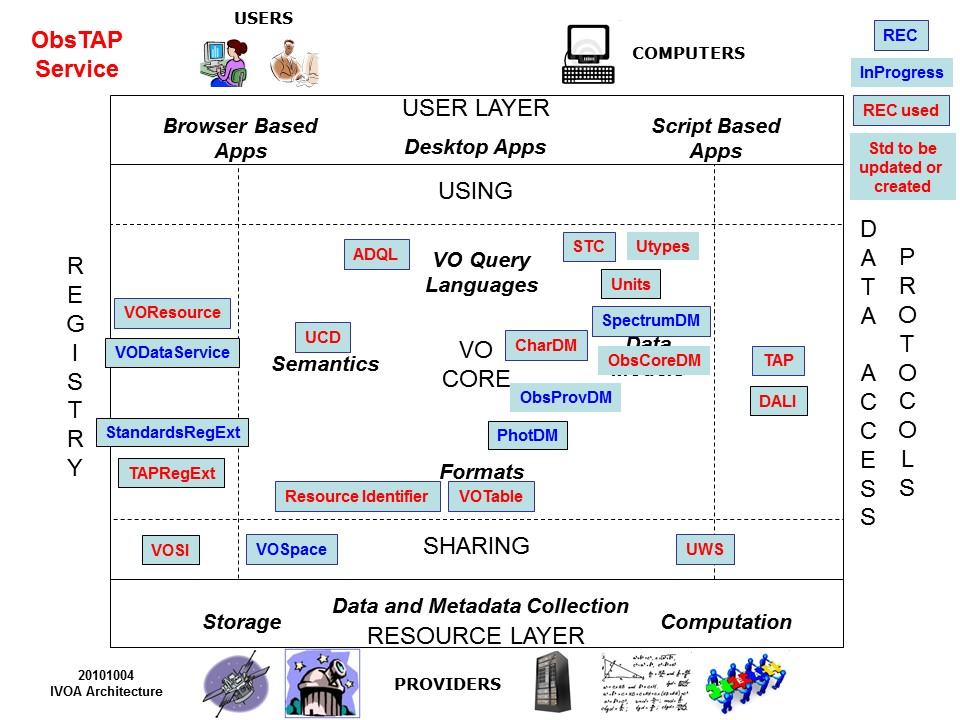
\includegraphics[width=0.9\textwidth]{role_diagram.jpg}
\caption{Architecture of an ObsTAP service}
\label{fig:archdiag}
\end{figure}
The architecture of an ObsTAP service: it is based on the ObsCore data model,
which re-uses parts of Characterisation, Spectrum, STC data models and the UCD and Units specifications. As a service
ObsTAP relies on ADQL, TAP, UWS, TAPRegExt, VOSI and VOTable. Examples and use-cases are exposed following the
recommendation for DALI examples.


\subsection{Second building block: the Table Access Protocol (TAP)}
TAP defines a service protocol for accessing tabular data such as astronomical catalogs, or more generally, database
tables.  TAP allows a client to (step 1) browse through the various tables and columns (names, units, etc.) in an
archive to collect the information necessary to pose a query, then (step 2) actually perform a table query.  The Table
Access Protocol (TAP) specification was developed and reached recommendation status in March 2010
\citep{2010ivoa.spec.0327D}.

\subsection{The goal of this effort}
Building on the work done on data models and TAP, it becomes possible to define a standard service protocol to expose
standard metadata describing available datasets.  In general, any data model can be mapped to a relational database and
exposed directly with the TAP protocol.  The goal of ObsTAP is to provide such a capability based upon an essential
subset of the general observational data model.

Specifically, this effort aims at defining a database table to describe astronomical datasets (data products) stored in
archives that can be queried directly with the TAP protocol.  This is ideal for global data discovery as any type of
data can be described in a straightforward and uniform fashion.  The described datasets can be directly downloaded or
accessed via IVOA Data Access Layer (DAL) protocols. 

The final capability required to support uniform global data discovery and access, with a client sending one and the
same query to multiple TAP services, is the stipulation that a uniform standard data model is exposed (through TAP)
using agreed naming conventions, formats, units, and reference systems.  Defining this core data model and associated
query mechanism is what this document is for.  

Thus the purpose of this document is twofold: (1) to define a simple data model to describe observational data, and (2)
to define a standard way to expose it through the TAP protocol to provide a uniform interface to discover observational
science data products of any type.

This document is organized as follows:
\begin{itemize}
\item Section \ref{sec:use-cases} briefly presents the types of the use cases collected from the astronomical
community by the IVOA Uptake committee. 
\item Section \ref{sec:core-components} defines the core components of the Observation data model. The elements of the data
model are summarized in Figure \ref{fig:obsdataset}. Mandatory ObsTAP fields are summarized in Table 1.
\item Section \ref{sec:obstap-impl} specifies the required data model fields as they are used in the TAP service: table
names, column names, column data type, UCD, Utype from the Observation Core components data model, and required units. 
\item Section \ref{sec:obstap-register} describes how to register an ObsTAP service in a Virtual Observatory registry. 
More detailed information is available in the appendices.
\item Examples are cited in Appendix A
\item Section 6 summarizes updates of this document.
\item Appendix A describes all the use cases as defined by the IVOA Take Up Committee.
\item Appendix B contains a full description of the Observation data model Core Components.
\item Appendix C shows the detailed content of the TAP\_SCHEMA tables and how to build up and fill them for the
implementation of an ObsTAP service.
\end{itemize}

\section[Use cases]{Use cases}
\label{sec:use-cases}Our primary focus is on data discovery.  To this end a number of use-cases have been defined,
aimed at finding observational data products in the VO domain by broadcasting the same query to multiple archives
(global data discoverability and accessibility).  To achieve this we need to give data providers a set of metadata
attributes that they can easily map to their database system in order to support queries of the sort listed below.

The goal is to be simple enough to be practical to implement, without attempting to exhaustively describe every
particular dataset.

The main features of these use-cases are as follows: 

\begin{itemize}
\item Support multi-wavelength as well as positional and temporal searches.
\item Support any type of science data product (image, cube, spectrum, time series, instrumental data, etc.).
\item Directly support the sorts of file content typically found in archives (FITS, VOTable, compressed files,
instrumental data, etc.).
\end{itemize}
Further server-side processing of data is possible but is the subject of other VO protocols.  More refined or advanced
searches may include extra knowledge obtained by prior queries to determine the range of data products available.

The detailed list of use cases proposed for data discovery is given in Appendix A.

%\subsection{Role within the VO Architecture}

%\begin{figure}
%\centering
% As of ivoatex 1.2, the architecture diagram is generated by ivoatex in
% SVG; copy ivoatex/archdiag-full.xml to role_diagram.xml and throw out
% all lines not relevant to your standard.
% Notes don't generally need this.  If you don't copy role_diagram.xml,
% you must remove role_diagram.pdf from SOURCES in the Makefile.

%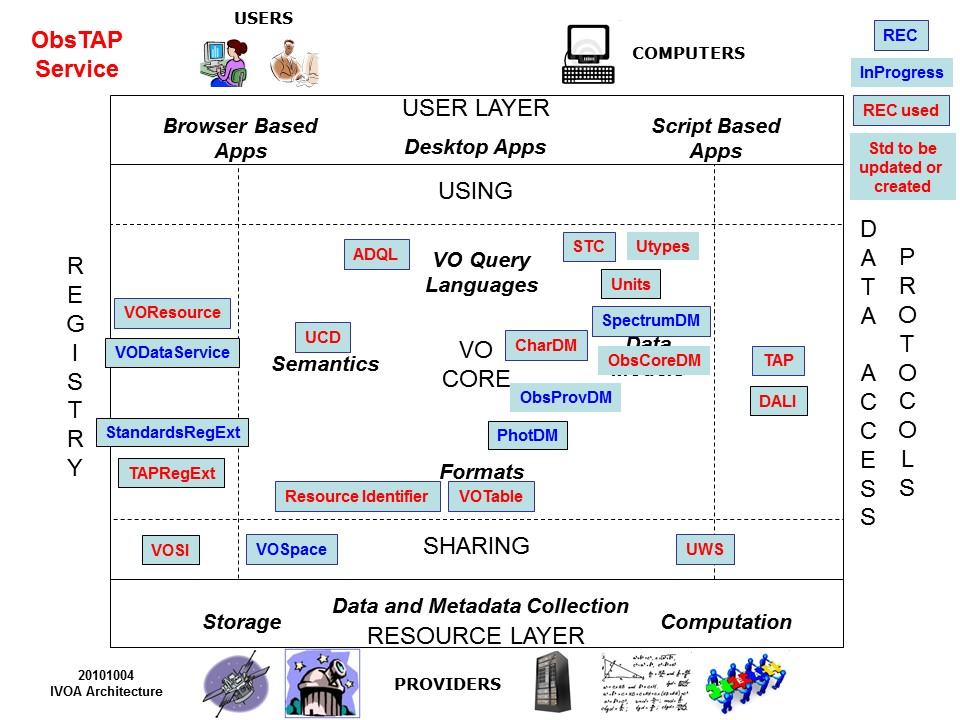
\includegraphics[width=0.9\textwidth]{role_diagram.pdf}
%\caption{Architecture diagram for this document}
%\label{fig:archdiag}
%\end{figure}
%Fig.~\ref{fig:archdiag} shows the role this document plays within the
%IVOA architecture \citep{2021ivoa.spec.1101D}.

\section[Observation Core Components Data Model]{Observation Core Components Data Model}
\label{sec:core-components}This section highlights and describes the core components of the Observation data model,
synthetized today in the Dataset Metadata DM specification. The term ``core components'' is meant to refer to those
elements of the larger ``Observation Data Model'' that are required to support the use cases listed in Appendix A.  In
reality this effort is the outcome of a trade-off between what astronomers want and what data providers are ready to
offer.  The aim is to achieve buy-in of data providers with a simple and {\textquotedbl}good enough{\textquotedbl}
model to cover the majority of the use cases.

The project of elaborating a general data model for the metadata necessary to describe any astronomical observation was
launched at the first Data Model WG meeting held in Cambridge, UK at the IVOA meeting in May 2003. The first
Observation data model was sketched out relying on some key concepts: Dataset, Identification, Curation, physical
Characterisation and Provenance (either instrumental or software).  A description of the early stages of this
development can be found in \citep{IVOANote:DMObservation} (Observation IVOA note). Some of these concepts have already
been elaborated in existing data models, namely the Spectrum data model \citep{2011ivoa.spec.1120M}  for general items
such as dataset identification and curation, and the Characterisation data model \citep{2008ivoa.spec.0325L} for the
description of the physical axes and properties of an observation, such as coverage, resolution, sampling, and
accuracy.  The Core Components data model reuses the relevant elements from those models.  Generalization of the
observational model to support data from theoretical models (e.g., synthetic spectra) is possible but is not addressed
here in order to keep the core model simple.

\subsection[UML description of the model]{UML description of the model}
\label{sec:uml}
This section provides a graphical overview of the Observation Core Components data model using the unified modeling
language (UML).  The UML class diagram shown in Figure 2 depicts the overall Observation Data Model, detailing those
aspects that are relevant to the Core Components, while omitting those not relevant.  The Characterisation classes
describing how the data span along the main physical measurement axes are simplified here showing only the attributes
necessary for data discovery.  This is also the case for the DataID and Curation classes extracted from the
Spectrum/SSA data model where only a subset of the attributes are actually necessary for data discovery.  For our
purposes here we show Characterisation classes only down to the level of the Support class (level 3).

\begin{figure}[H]
\centering
%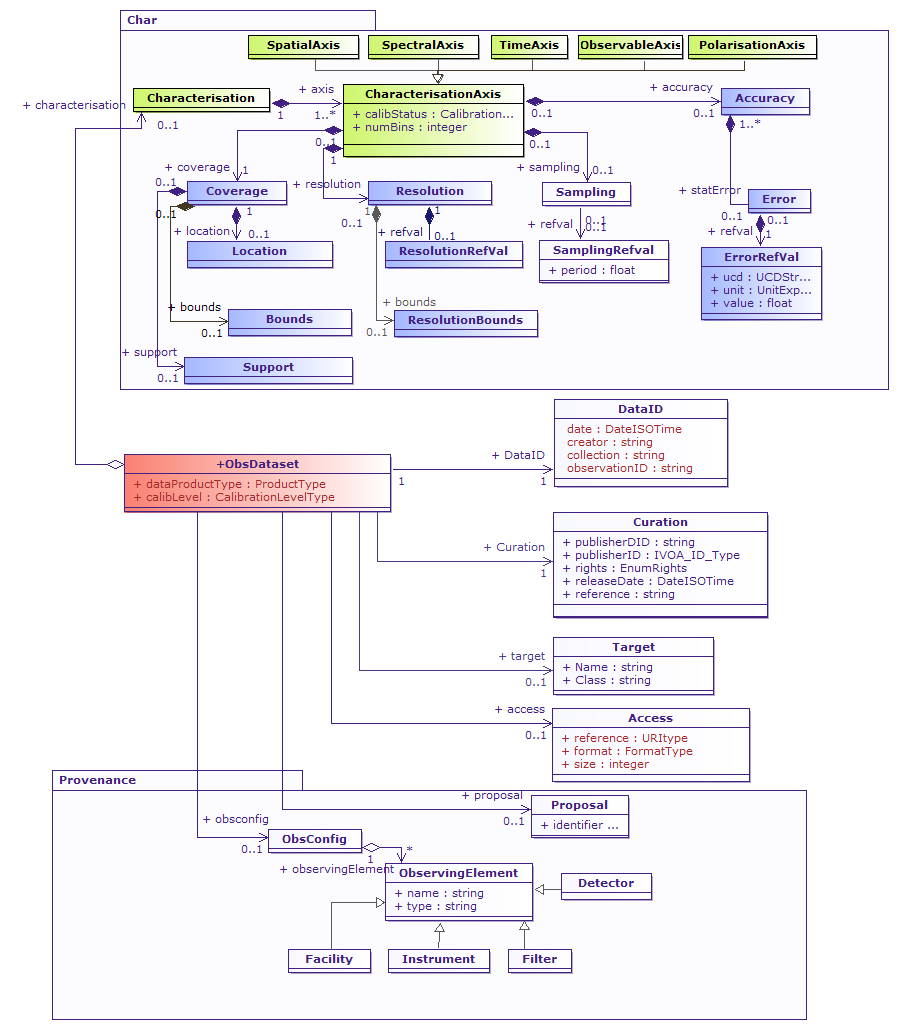
\includegraphics[width=17.489cm,height=19.59cm]{ObsDataset.png}
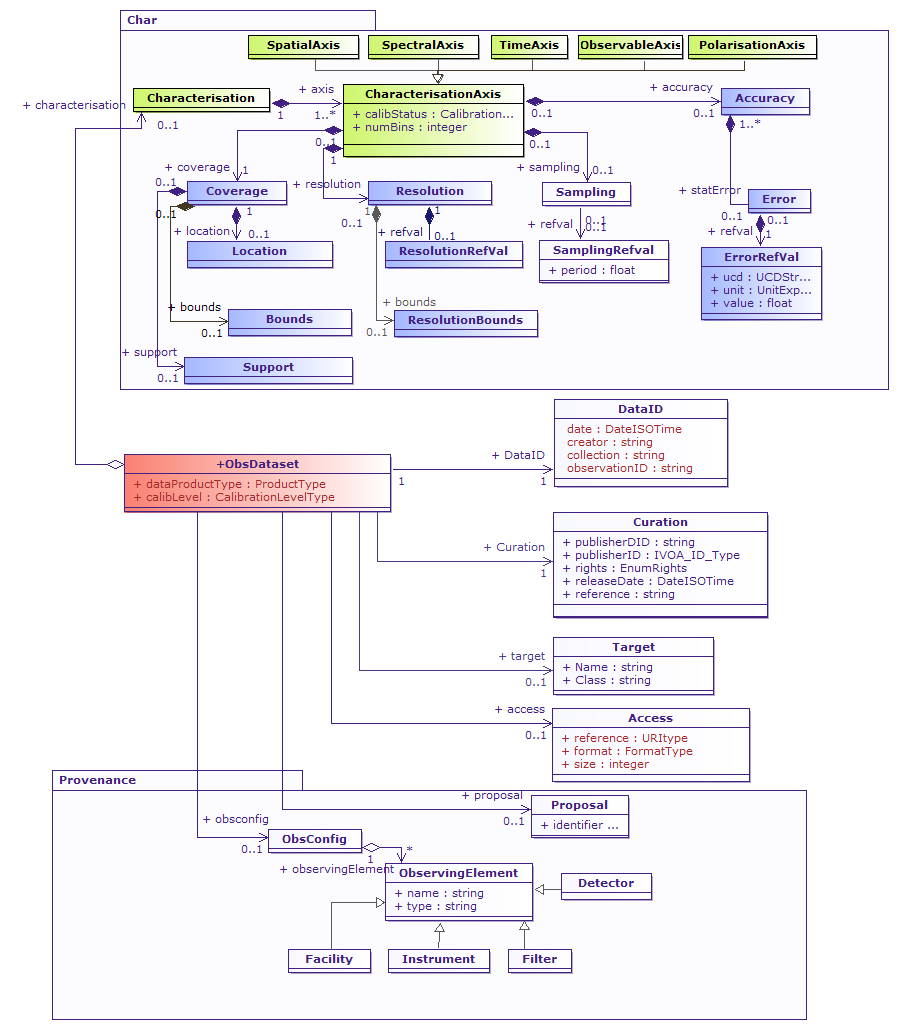
\includegraphics[width=0.9\textwidth]{ObsDataset.png}
\caption{ObsDataset metadata}
\label{fig:obsdataset}
\end{figure}
Figure \ref{fig:obsdataset} depicts the classes used to organize observational metadata. Classes may be linked either via 
association or aggregation.  The minimal set of necessary attributes for data discovery is shown in brown.

For the sake of clarity, the SpatialAxis, SpectralAxis and TimeAxis classes on the diagram are not expanded on the main
class diagram. Details for these axes are shown in Figure 3 for the spatial axis, Figure 4 for the spectral axis and
Figure 5 for the time axis.

\begin{figure}[H]
\centering
%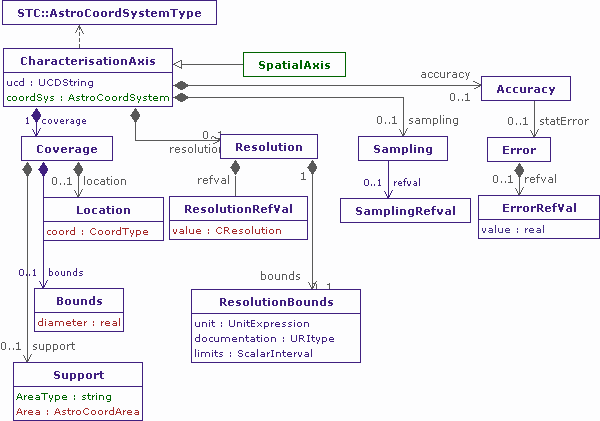
\includegraphics[width=14.605cm,height=10.239cm]{Char-Spatial.png}
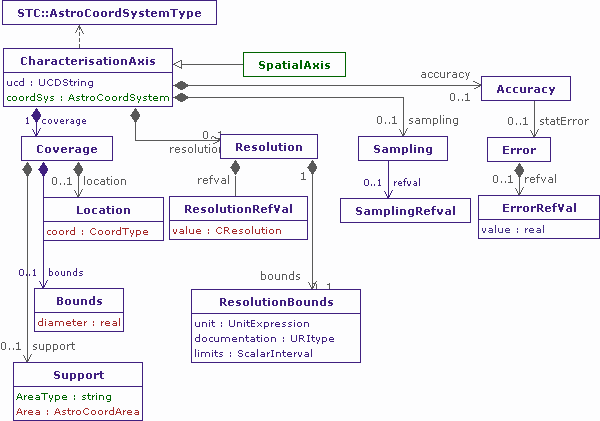
\includegraphics[width=0.9\textwidth]{Char-Spatial.png}
\caption{Spatial Axis Characterisation}
\label{fig:char-spatial}
\end{figure}
Figure \ref{fig:char-spatial} shows the details of the classes linked to the description of the
spatial axis for an Observation dataset. All axes in this model inherit the main structure from the
CharacterisationAxis class, but some peculiar attributes are necessary for Space coordinates.

\begin{figure}[H]
\centering
%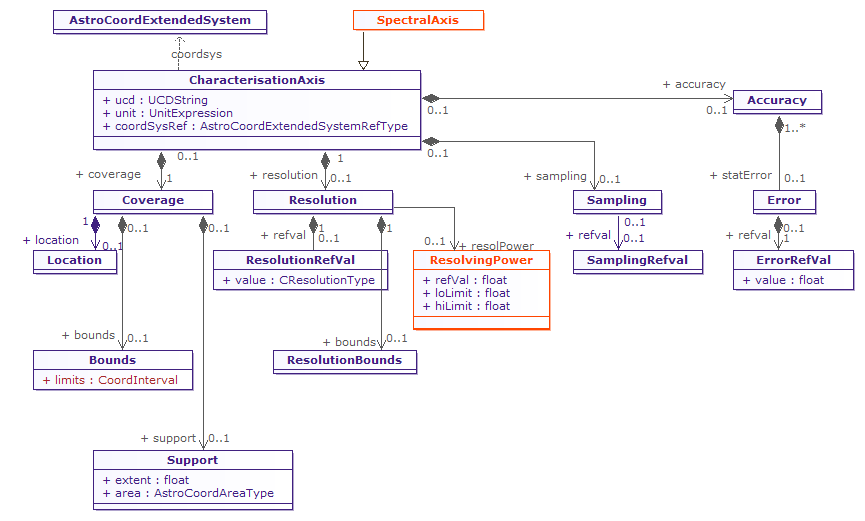
\includegraphics[width=17.427cm,height=10.495cm]{Char-Spectral.png}
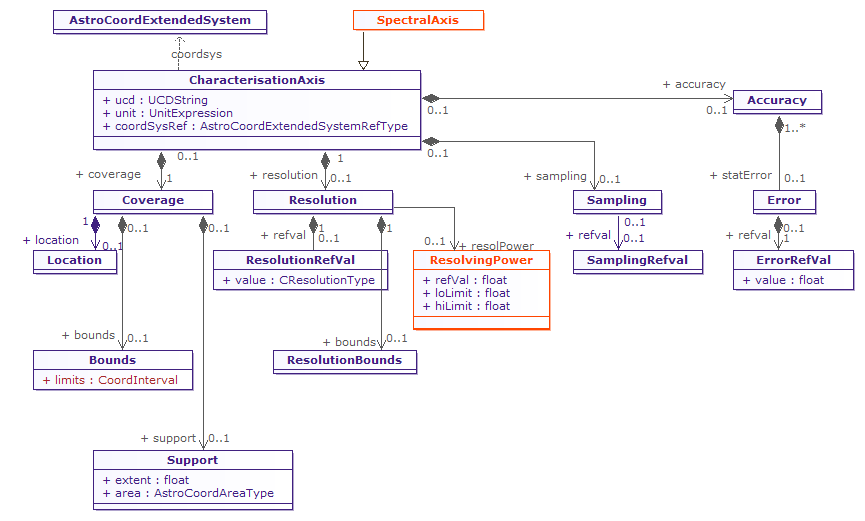
\includegraphics[width=0.9\textwidth]{Char-Spectral.png}
\caption{Spectral Axis Characterisation}
\label{fig:char-spectral}
\end{figure}
Figure \ref{fig:char-spectral} shows the Spectral axis: details of the classes necessary to
describe the spectral properties of an Observation dataset. UCD and units are essential to disentangle various possible
spectral quantities.

\begin{figure}[H]
\centering
%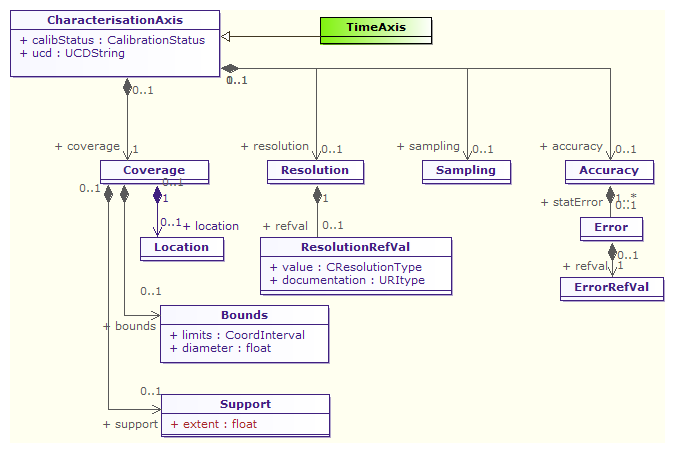
\includegraphics[width=13.524cm,height=9.075cm]{Char-Time.png}
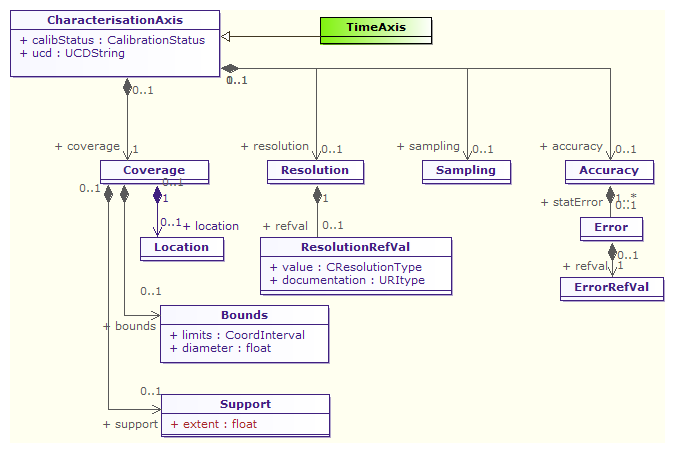
\includegraphics[width=0.9\textwidth]{Char-Time.png}
\caption{Time Axis Characterisation}
\label{fig:char-time}
\end{figure}
Figure \ref{fig:char-time} shows the classes from the Characterisation DM used to
describe time metadata.

Details on the ObsCoreDM axes definitions are available in the Characterisation data model standard document
\citep{2008ivoa.spec.0325L}. The hypertext documentation of the model is available on the IVOA web site under the
ObsCore wiki page  \url{http://www.ivoa.net/internal/IVOA/ObsDMCoreComponents/} .

\subsection[Main Concepts of the ObsCore Data Model]{Main Concepts of the ObsCore Data Model}
The ObsCore data model is the result of the analysis of the data discovery use cases introduced in Chapter 2. Two sets
of elements have been identified: those necessary to support the provided use cases, and others that are generally
useful to describe the data but are not immediately required to support the use cases.  In this section only the first
set is described.  That set coincides with the set of parameters that any ObsTAP service must support. Please refer to
appendix B for the detailed description of all model elements. 

Table 1 lists the data model elements that any ObsTAP implementation must support (i.e. a column with such name must
exist, though, in some cases, it could be nillable).  Provision of these mandatory fields ensures that any query based
on these parameters is guaranteed to be understood by all ObsTAP services.

NB: Data model fields are listed here with their TAP column name rather than the IVOA data model element identifiers
(Utype) to ease readability.  See the associated Utypes in Appendix C. 

%\begin{table}[h]
%\begin{center}
\begin{longtable}{|l|p{0.2\textwidth}|p{0.2\textwidth}|p{0.2\textwidth}|p{0.35\textwidth}|}
\hline
Column Name & Unit & Type & Description\\\hline
dataproduct\_type & unitless & String & Logical data product type (image etc.)\\\hline
calib\_level & unitless & enum integer  & Calibration level \{0, 1, 2, 3, 4\} \\\hline
obs\_collection & unitless & String & Name of the data collection \\\hline
obs\_id & unitless & String & Observation ID \\\hline
obs\_publisher\_did & unitless & String & Dataset identifier given by the publisher\\\hline
access\_url & unitless & String & URL used to access (download) dataset\\\hline
access\_format & unitless & String & File content format (see in App. \ref{bkm:Ref297463580} )\\\hline
access\_estsize & kbyte & integer & Estimated size of dataset in kilo bytes\\\hline
target\_name & unitless & String & Astronomical object observed, if any\\\hline
s\_ra & deg & double & Central right ascension, ICRS\\\hline
s\_dec & deg & double & Central declination, ICRS\\\hline
s\_fov & deg & double & Diameter (bounds) of the covered region \\\hline
s\_region & unitless & String & Sky region covered by the  data product (expressed in ICRS frame)\\\hline
s\_xel1 & unitless & integer & Number of elements along the first spatial axis\\\hline
s\_xel2 & unitless & integer & Number of elements along the second spatial axis\\\hline
s\_resolution & arcsec & double & Spatial resolution of data as FWHM\\\hline
t\_min & d & double & Start time in MJD\\\hline
t\_max & d & double & Stop time in MJD\\\hline
t\_exptime & s &  double & Total exposure time\\\hline
t\_resolution & s & double & Temporal resolution\\\hline
t\_xel & unitless & integer & Number of elements along the time axis\\\hline
em\_min & m & double & Start in spectral coordinates\\\hline
em\_max & m & double & Stop in spectral coordinates\\\hline
em\_res\_power & unitless & double & Spectral resolving power\\\hline
em\_xel & unitless & integer & Number of elements along the spectral axis\\\hline
o\_ucd & unitless & String & UCD of observable (e.g. phot.flux.density, phot.count, etc.)\\\hline
pol\_states & unitless & String & List of polarization states or NULL if not applicable\\\hline
pol\_xel & unitless & integer & Number of polarization samples \\\hline
facility\_name & unitless & String & Name of the facility used for this observation \\\hline
instrument\_name & unitless & String & Name of the instrument used for this observation \\\hline
\end{longtable}
%\end{center}
\label{bkm:Ref460858868}Table T1.  Mandatory fields of the Observation Core Components data
model with their name, recommended units, data type and designation.
%\end{table}

\subsection{Specific Data Model Elements}
In order to support the global data discoverability and accessibility requirements, some new concepts previously not
covered by any other data model have to be introduced.  This section describes those, which are: the data product type,
a classification of the various levels of calibration and processing applied to the data, the file content and format
enriched and extended from the concept described in the SSA protocol\citep{2012ivoa.spec.0210T}.  In addition, a
clarification of how the terms Observation and Data Product are used in the ObsTAP context is provided as well as a
discussion for composed products.

\subsubsection{Data Product Type}
\label{bkm:Ref286875933}The model defines a data product type attribute to describe the high level scientific
classification of the data product being considered.  This is coded as a string that conveys a general idea of the
content and organization of a dataset.  We consider a coarse classification of the types of dataset interesting for
science usage, covering: image, cube, spectrum, SED, time series, visibility data, and event data.

\begin{itemize}
\item image An astronomical image, typically a 2D image with two spatial axes, e.g., a FITS image.  The image content
may be complex, e.g., an objective-grism observation would be considered a type of image, even though an extracted
spectrum would be a Spectrum data product.
\item cube  A multidimensional astronomical image with 3 or more image axes, e.g., a spectral image cube, a polarization
cube, a full Stokes radio data cube, a time image cube, etc.  The most common format for astronomical ``cube'' data
products is a multidimensional FITS image, however other formats are allowed so long as they are adequately described.
\item spectrum Any dataset for which spectral coverage is the primary attribute, e.g., a 1D spectrum or a long slit
spectrum.
\item sed  A spectral energy distribution, an advanced data product often produced by combining data from multiple
observations.
\item timeseries A one dimensional array presenting some quantity as a function of time.  A light curve is a typical
example of a time series dataset.
\item visibility A visibility (radio) dataset of some sort.  Typically this is instrumental data, i.e.,
{\textquotedbl}visibility data{\textquotedbl}.  A visibility dataset is often a complex object containing multiple
files or other substructures.  A visibility dataset may contain data with spatial, spectral, time, and polarization
information for each measured visibility, hence can be used to produce higher level data products such as image,
spectra, timeseries, and so forth.
\item event An event-counting (e.g. X-ray or other high energy) dataset of some sort.  Typically this is instrumental
data, i.e., {\textquotedbl}event data{\textquotedbl}.  An event dataset is often a complex object containing multiple
files or other substructures.  An event dataset may contain data with spatial, spectral, and time information for each
measured event, although the spectral resolution (energy) is sometimes limited.  Event data may be used to produce
higher level data products such as images or spectra.
\item measurements A list of derived measurements gathered in a particular original dataset of one of the previous sort
after some analysis processing, like a source list, or more generally a list of `results' attached to such datasets.
\end{itemize}
Classification of astronomical data by data product type is inherently ambiguous hence the classification scheme defined
here is intentionally kept as simple as possible.  The data provider should pick the primary category most appropriate
for their data. Values must be specified in lower-case (in order to simplify queries).  One of the defined
dataproduct\_type values must be used if appropriate for the data product in question, otherwise a NULL value is
permitted and a more precise definition of the data product type should be given in dataproduct\_subtype. Combination
of data product types is not allowed, i.e., either one of the above values or NULL must be specified.

Further information on the specific content of a data product can be provided by the dataproduct\_subtype data model
field defined in the data model appendix \ref{bkm:Ref291536287} , and by the related obs\_title
(\ref{bkm:Ref292046860}) and access\_format attributes (section \ref{bkm:Ref289893457}). 

The intent of dataproduct\_type is to provide only a general indication of the category to which the data product
belongs to facilitate global data discovery.

\subsubsection{Calibration level}
\label{bkm:Ref158638048}\label{bkm:Ref287048333}The calibration level concept conveys to the user information on how
much data reduction/processing has been applied to the data.  It is up to the data providers to consider how to map
their own internal classification to the suggested classification scale here.

Level 0:  Raw instrumental data, in a proprietary or internal data-provider defined format, that needs instrument
specific tools to be handled. 

Level 1:  Instrumental data in a standard format (FITS, VOTable, SDFITS, ASDM, etc.) which could be manipulated with
standard astronomical packages.

Level 2: Calibrated, science ready data with the instrument signature removed.

Level 3: Enhanced data products like mosaics, resampled or drizzled images, or heavily processed survey fields.  Level 3
data products may represent the combination of data from multiple primary observations.

Level 4: Analysis data products generated after some scientific data manipulation or interpretation. 

The examples in the following subsection should help illustrate use of the calib\_level attribute. It is left to the
data provider to decide for ambiguous cases.

\paragraph[Examples of datasets and their calibration level]{Examples of datasets and their calibration level}
Here are examples of various datasets, classified according to scheme defined above. 

%\begin{table}[h]
%\begin{center}
\begin{tabular}{|l|p{0.2\textwidth}|p{0.2\textwidth}|p{0.2\textwidth}|p{0.35\textwidth}|}
\hline
Data product type & Data collection & Calibration Level & Comments\\\hline
image & IRAS/NASA & 2 & Science ready data\\\hline
image & IRIS/IRSA & 3 & Recalibrated from infrared IRAS images with removal of the sensor memory effect.\\\hline
image & HDFS/ACS GOODS data & 3 & Image associations mosaicking/stacking\\\hline
spectrum & XMM-Newton EPIC spectra & 1 & Raw instrumental spectrum.\\\hline
cube & EVLA spectral data cube & 2 & Radio spectral data cube in FITS format\\\hline
sed & NED SED & 3 & NED spectral energy distribution\\\hline
event & ROSAT/HEASARC & 1 & Instrumental data\\\hline
visibility & ALMA, Merlin, etc. & 1 & Instrumental data\\\hline
measurements & ESO tile catalog  & 4 & Photometric catalog of extracted sources for a tile image\\\hline
timeseries & CTA reconstructed light curve  & 4 & Reconstructed light curve following photons vs particles separation under some assumption \\\hline
\end{tabular}
%\end{center}
\label{T2}Table T2. Examples of datasets with their associated calibration level values.
%\end{table}

\subsubsection{Observation and Observation Dataset}
\label{bkm:Ref450327253}ObsTAP describes observations in a broad sense; exactly what comprises an
{\textquotedbl}observation{\textquotedbl} is not well defined within astronomy and is left up to the data provider to
define for their data.  ObsTAP also describes archive data products (e.g., actual archive files). 

The IVOA Dataset Metadata model (see http://www.ivoa.net/documents/DatasetDM/) clarifies the logical links between an
Observation and an ObservationDataset i.e a data product here. It makes a distinction between an
{\textquotedbl}observation{\textquotedbl} as the description of an observing experiment and its resulting datasets.
Therefore the term ObsDataset is adopted in this version as a replacement of Observation in the previous ObsCore1.0
specification. It helps to handle various situations of combination, stacking, packaging of the results of performing
an observation at the instrument level. 

In general an Observation Dataset, as a result, may be composed of multiple individual data products.  In this case all
the data products stemming from one observation should share the same observation identifier (obs\_id).  The form of
the obs\_id string is up to the data provider so long as it uniquely identifies, within the context of the archive, all
data products resulting from the observation.  The individual data products associated with an observation may have
different data product types, calibration levels, and so forth.  ObsTAP only directly supports the description of
science data products, i.e., data products which contain science data having some physical (spatial, spectral,
temporal) coverage.

Two different approaches can be followed for exposing the instrumental data from an observation. One can either expose
the individual science data products resulting from the observation, all sharing the same obs\_id, or one can
``package'' the data products and expose the package as a single complex instrumental data product. Combinations of the
two approaches are also possible, e.g., a package of all the data products, plus additional records exposing selected
high priority individual data products, all sharing the same obs\_id.

If the data products comprising an observation are exposed individually then attributes such as the calibration level
can vary for different data products, e.g., the raw instrumental data as observed might be level 1, a standard pipeline
data product might be level 2, and a custom user-processed data product subsequently published back to the archive
might be level 3.  All such data products would share the same obs\_id.

If on the other hand all data from an observation is exposed as a single data product via ObsTAP this will likely be an
aggregate of some sort (tar file, directory, etc.) containing multiple files.  This latter approach is limited to
instrumental data (level 0 or 1), even if objects within the aggregate observation file are higher level.  From the
perspective of ObsTAP this would be instrumental data, and it is up to the user or client application consuming the
data to interpret the meaning of the data elements within the observation.

Which approach is best depends upon the anticipated scientific usage and is up to the data provider to determine.  For
example if the observational data provided is most commonly used for multi-wavelength analysis, exposing individual
high level data products is likely to be the best approach.  If the anticipated usage is dominated by complex analysis
of instrumental data, then exposing the entire observation as a standard package of instrumental data may be preferred.

\subsubsection{File Content and Format}
While dataproduct\_type specifies at a high level what a specific data product is, the access\_format attribute
specifies what is actually in the file.  For example, an {\textquotedbl}image{\textquotedbl} could be a FITS image, an
image embedded in a FITS multi-extension format (MEF) file, a JPEG, etc.  A {\textquotedbl}spectrum{\textquotedbl}
could be represented in the VO-compliant Spectrum format, or in some instrument-specific FITS binary table format.  A
visibility dataset could be in FITS or ASDM format, or a variety of other radio data formats.  A ROSAT or Chandra
observation might be presented as a `tar' file or directory containing instrument-specific observational files.  There
are many such examples; we give only a few here to illustrate the concept.

Specifying the content and format of a data product is important as special software may be required to do anything
useful with the data.  The user needs to know exactly what the data product is before deciding to download it for
analysis. 

See section \ref{bkm:Ref289893457} for more details and implementation requirements.

\section{Implementation of ObsCore in a TAP Service}
\label{sec:obstap-impl}The ObsCore model must be implemented within Table Access Protocol (TAP) services such that all
valid queries can be executed unchanged on any service that implements the model.  Additional optional or
provider-defined columns are permitted (see section \ref{bkm:Ref421295535}) so long as all mandatory columns are
provided.  The protocol does not specify any specific ordering of fields in the query response so long as the mandatory
parameters are present in the output stream.

Here we specify an explicit mapping of the model to relational database tables; in the context of TAP this means we are
specifying the logical tables as described in the TAP\_SCHEMA (the TAP-required database schema where the tables and
columns exposed by the service are described).  This does not necessarily imply that the underlying database will have
the identical structure (what is exposed through TAP could be, for example, a database view of the underlying database
tables), but in most cases the relationship between TAP\_SCHEMA description and the underlying tables is
straightforward.

%\begin{table}[h]
%\begin{center}
\begin{tabular}{|p{0.2\textwidth}|p{0.2\textwidth}|p{0.6\textwidth}|}
\hline
schema\_name & table\_name & Description\\\hline
ivoa & ivoa.ObsCore & ObsCore 1.1\\\hline 
\end{tabular}
%\end{center}
\label{T3}Table T3. TAP\_SCHEMA.tables for implementation of the ObsCore model.
%\end{table}

%\begin{table}[h]
%\begin{center}
\begin{longtable}{|p{0.20\textwidth}|p{0.28\textwidth}|p{0.22\textwidth}|p{0.1\textwidth}|p{0.20\textwidth}|}
\hline
table\_name & column\_name & data type & units & Constraint\\\hline
ivoa.ObsCore & dataproduct\_type & adql:VARCHAR &  & \\\hline
ivoa.ObsCore & calib\_level & adql:INTEGER & & not null\\\hline
ivoa.ObsCore & obs\_collection & adql:VARCHAR & & not null\\\hline
ivoa.ObsCore & obs\_id & adql:VARCHAR & & not null\\\hline
ivoa.ObsCore & obs\_publisher\_did & adql:VARCHAR & & not null\\\hline
ivoa.ObsCore & access\_url & adql:CLOB & & \\\hline
ivoa.ObsCore & access\_format & adql:VARCHAR & & \\\hline
ivoa.ObsCore & access\_estsize & adql:BIGINT & kbyte & \\\hline
ivoa.ObsCore & target\_name & adql:VARCHAR & & \\\hline
ivoa.ObsCore & s\_ra & adql:DOUBLE & deg & \\\hline
ivoa.ObsCore & s\_dec & adql:DOUBLE & deg  & \\\hline
ivoa.ObsCore & s\_fov & adql:DOUBLE & deg  & \\\hline
ivoa.ObsCore & s\_region & adql:REGION &  & \\\hline
ivoa.ObsCore & s\_resolution & adql:DOUBLE & arcsec  & \\\hline
ivoa.ObsCore & s\_xel1 & adql:BIGINT &  & \\\hline
ivoa.ObsCore & s\_xel2 & adql:BIGINT &  & \\\hline
ivoa.ObsCore & t\_min & adql:DOUBLE & d  & \\\hline
ivoa.ObsCore & t\_max & adql:DOUBLE & d  & \\\hline
ivoa.ObsCore & t\_exptime & adql:DOUBLE & s  & \\\hline
ivoa.ObsCore & t\_resolution & adql:DOUBLE & s  & \\\hline
ivoa.ObsCore & t\_xel & adql:BIGINT &  & \\\hline
ivoa.ObsCore & em\_min & adql:DOUBLE & m & \\\hline
ivoa.ObsCore & em\_max & adql:DOUBLE & m & \\\hline
ivoa.ObsCore & em\_res\_power & adql:DOUBLE & & \\\hline
ivoa.ObsCore & em\_xel & adql:BIGINT & & \\\hline
ivoa.ObsCore & o\_ucd & adql:VARCHAR & & \\\hline
ivoa.ObsCore & pol\_states  & adql:VARCHAR & & \\\hline
ivoa.ObsCore & pol\_xel & adql:BIGINT & & \\\hline
ivoa.ObsCore & facility\_name & adql:VARCHAR & & \\\hline
ivoa.ObsCore & instrument\_name & adql:VARCHAR & & \\\hline
\end{longtable}
%\end{center}
\label{bkm:Ref286578377}Table T4. List of the minimal set of data model fields to
implement for an ObsTAP service. See tables of Appendix C for the full description of the TAP\_SCHEMA.columns table. 
%\end{table}

Table 3 and Table 4 provide the primary information needed to describe the ObsCore model in terms of TAP\_SCHEMA tables
and columns. 

The ``datatype'' column values should follow the TAP standard specification and are bound to the TAP specification
version used to implement the model. Here what is shown applies for TAP v1.0. 

The content of the ``constraint'' column specified in Table 4 above is not part of the TAP\_SCHEMA.columns description,
but is required by the ObsCore model and specified here to make this clear to implementers.  Additional standard
content for the individual columns is specified below. 

\subsection{Data Product Type (dataproduct\_type)}
The dataproduct\_type column contains a simple string value describing the primary nature of the data product.  It
should assume one of these string values: image, cube, spectrum, sed, timeseries, visibility, event or measurements. 
These values are described in section \ref{bkm:Ref286875933}.  A NULL value is permitted, but only in the event that
none of the proposed values can be used to describe the dataset.  The optional field dataproduct\_subtype
(\ref{bkm:Ref291536287}) may be used to more precisely define the nature of the dataset.  Values in the
dataproduct\_type column must be written in lower case. Specifying this field along with the desired spatial and
spectral coverage will be enough to discover data of interest in many common cases. 

Usage: select * from ivoa.ObsCore where dataproduct\_type='image' returns only image data.

\subsection{ Caveat while using dataproduct\_type=``measurements''}
Note that ``measurements'' extends the set of accepted values for dataproduct\_type in ObsCore 1.0. This extension is
meant to expose derived data products together with the progenitor observation dataset. 

A few mandatory keywords for the axes description may be non-applicable for such a data product. In this case the
coverage on spatial, energy, time, and polarization may inherit the values from the ObsCore description of its
progenitor. 

Progenitors and their derived data products must have the same obs\_id.

\subsection{Calibration Level (calib\_level)}
The calib\_level column tells the user the amount of calibration processing that has been applied to create the data
product. calib\_level must assume one value among \{0, 1, 2 ,3, 4\}. Please refer to section \ref{bkm:Ref287048333} for
a full description of the various categories.  Data providers decide which value best describes their data products.

Values in the calib\_level column must not be NULL.

Query usage: ``select * from ivoa.ObsCore where calib\_level {\textgreater}2'' returns enhanced data products.

\subsection{Collection Name (obs\_collection)}
The obs\_collection column identifies the data collection to which the data product belongs.  A data collection is any
logical collection of datasets which are alike in some fashion.  Typical data collections might be all the data from a
particular telescope, instrument, or survey. The value is either the registered shortname for the data collection, the
full registered IVOA identifier for the collection, or a data provider defined shortname for the collection.  Often the
collection name will be set to the name of the instrument that generated the data.  In that case we suggest specifying
the collection name as a string composed of the facility name, followed by a slash, followed by the instrument name. 

Examples : HST/WFPC2, VLT/FORS2, CHANDRA/ACIS-S. 

There are other cases where it makes no sense to use the instrument name, may be because the data product used data from
different instruments or facilities, or for other reasons.  Examples: SDSS-DR7, etc.

In practice this is not a very precisely defined field.  What is important is for the data provider to use a collection
name which is familiar to astronomers and discriminative to point easily on datasets of interest.  

Values in the obs\_collection column must not be NULL.

\subsection{Observation Identifier (obs\_id)}
The obs\_id column defines a unique identifier for an observation as explained in section \ref{bkm:Ref450327253} . In
the case where multiple data products are available for an observation (e.g. with different calibration levels), the
obs\_id value will be the same for each data product comprising the observation. This is equivalent to the dataset name
for many archives where dataset name could have many files associated with them. The returned obs\_id for an archival
observation should remain identical through time for future reference.

In the case of some advanced data products (with calib\_level ${\geq}$ 3), the data product may be the result of
combining data from multiple primary (physical) observations.  In this case the resulting data product is a new
processed ``observation'' to which a new unique observation identifier should be assigned.  If the advanced processing
results in several associated data products they should share the same obs\_id.  Describing the provenance of such an
advanced data product is possible, but is out of scope for ObsTAP.

Values in the obs\_id column must not be NULL.

\subsection{Publisher Dataset Identifier (obs\_publisher\_did)}
The obs\_publisher\_did column contains the IVOA dataset identifier \citep{2007ivoa.spec.0314P} for the published data
product.  This value must be unique within the namespace controlled by the dataset publisher (data center).  The value
will also be globally unique since each publisher has a unique IVOA registered publisher ID.  The same dataset may
however have more than one publisher dataset identifier if it is published in more than one location; the creator DID,
if defined for the given dataset, would be the same regardless of where the data is published.

The returned obs\_publisher\_did for a static data product should remain identical through time for future reference.

Values in the obs\_publisher\_did column must not be NULL.

\subsection{Access URL (access\_url)}
The access\_url column contains a URL that can be used to download the data product (as a file of some sort).

We specify the data type as CLOB (character large object) in the TAP service so that users will know they can only use
the access\_url column in the SELECT clause of a query.  That is, users cannot specify this column as part of a
condition in the WHERE clause and implementers are free to generate the URL on the fly during output (rather than being
forced to store it statically in the database).

More details are given on the use of CLOB data types for the TAP SCHEMA in the TAP Standard document
\citep{2010ivoa.spec.0327D}, section 2.5 Table upload.

Access URLs are not guaranteed to remain valid and unchanged indefinitely.  To access a specific data product after a
period of time (e.g., days or weeks) a query should be performed (e.g., using obs\_publisher\_did) to obtain a fresh
access URL.

\subsection{Access Format (access\_format)}
\label{bkm:Ref289893457}The access\_format column specifies the format of the data product if downloaded as a file. This
data model field is important both for data discovery and for the client to evaluate whether it will be able to
actually use the data product if downloaded.

MIME types are often used to specify file formats in existing protocols such as HTTP \citep{std:MIME_types}.  However
when dealing with astronomical observations as in ObsTAP services, more information about the format of the data is
required than can be specified by conventional MIME types.  For instance we might want to distinguish between various
formats like multi-extension FITS (e.g. for CCD mosaic instruments or MUSE IFU data), or ASDM (e.g. for ALMA or other
interferometry observations).  Even for something as fundamental to astronomy as FITS binary table there is currently
no standardized MIME type other than the generic application/FITS.

While standard MIME types are limited when it comes to describing the many data formats actually in use within
astronomy, they are ideal for specifying common file types such as HTML and XML, the various graphics file types, text,
PDF, and so forth, all of which can be used to describe aspects of observational data.  Furthermore the MIME type
scheme is extensible, allowing new formats which are not yet standardized to be specified.  Hence what we propose here
is to adopt the MIME type mechanism to describe the file format of a science data product, defining new custom types as
needed.  Note this is distinct from the science content which is specified by the data product type and subtype.  The
same content can potentially be represented in multiple formats hence these are distinct.

The following table illustrates some common astronomical file formats.  This list is by no means intended to be
comprehensive; rather it illustrates the approach while defining standard values for some common formats.  Some
randomly selected formats are included to illustrate the approach.  We can extend this list as experience is gained
using ObsTAP to describe actual data archives.

%\begin{table}[h]
%\begin{center}
\begin{tabular}{|p{0.3\textwidth}|p{0.15\textwidth}|p{0.5\textwidth}|}
\hline
MIME-type & Shortname & Definition\\\hline 
image/fits   & fits & Any multidimensional regularly sampled FITS image or cube\\\hline
image/jpeg   & jpeg & A 2D JPEG graphic image (likewise for GIF, PNG, etc.)\\\hline
application/fits & fits & Any generic FITS file\\\hline
application/x-fits-bintable & bintable & A FITS binary table (single BINTABLE extension)\\\hline
application/x-fits-mef & mef & A FITS multi-extension file (multiple extensions)\\\hline
application/x-fits-uvfits & uvfits & A FITS file in UVFITS format (likewise SDFITS etc.)\\\hline
application/x-fits-euro3d & euro3d & A FITS file in Euro3D format (multiobject spectroscopy)\\\hline
application/x-votable+xml & VOTable & Any generic VOTable file\\\hline
application/x-asdm  & asdm & ALMA science data model (final export format still TBD)\\\hline
application/pdf & pdf & Any PDF file\\\hline
text/html   & html & Text in HTML format\\\hline
text/xml & xml & Any generic XML file\\\hline
text/plain & txt & Any generic text file\\\hline
text/csv & csv & Tabular data in comma separated values format\\\hline
text/tab-separated-values & tsv & Tabular data in tab separated values format\\\hline
application/x-tar & tar & Multiple files archive in TAR format\\\hline
application/zip & zip & Multiple files archive in ZIP format\\\hline
application/x-directory & dir & Multiple files archive returned as a text list \\\hline
image/x-fits-gzip & fits & A GZIP-compressed FITS image\\\hline
image/x-fits-hcompress & fits & A FITS image using HCOMPRESS compression\\\hline
application/x-tar-gzip & gtar & A GZIP-compressed TAR file (x-gtar also sometimes used)\\\hline
application/x-votable+xml; content=datalink & datalink & A datalink response containing links to  data sets or services attached to the current dataset\\\hline
\end{tabular}
%\end{center}
\label{bkm:Ref286578377}Table T5: TODO: label from orig doc
%\end{table}
The value of access\_format should be a MIME type, either a standard MIME type, an extended MIME type from the above
table, or a new custom MIME type defined by the data provider.  The short names suggested here are not used directly by
access\_format.

Custom file formats should be specified using a MIME type such as
{\textquotedbl}application/x-{\textless}whatever{\textgreater}{\textquotedbl}.  This can be used for any file format
including custom binary file formats.

Observational datasets consisting of multiple instrument-specific files may be exposed in formats like
application/x-directory, application/x-tar or application/x-tar-gzip.  Details of the package content and how to access
inner data products are described in the IVOA Data Link specification \citep{2015ivoa.spec.0617D}. See the example
presented in section \ref{bkm:Ref303703299} .

Compression is inherent in some file formats, e.g., ZIP or JPEG.  In other formats it is optional and is indicated by
having multiple versions of the format, e.g. image/fits or image/x-fits-gzip for a GZIP-compressed FITS image (the
{\textquotedbl}x-{\textquotedbl} prefix is required for anything which is not a registered standard MIME type).

The access\_url field may also point to a datalink service. This is stipulated by the
`application/x-votable+xml;content=datalink' access format. 

This service will return a response containing attached files related to the discovered dataset (previews, tar
ball{\dots}).  It can also contain descriptions of services running operations on the dataset like cut-outs..

\subsection{Estimated Download Size (access\_estsize)}
The access\_estsize column contains the approximate size (in kilobytes) of the file available via the access\_url.  This
is used only to gain some idea of the size of a data product before downloading it, hence only an approximate value is
required.  Provision of dataset size estimates is important whenever it is possible that datasets can be very large. 

\subsection{Target Name (target\_name)}
The target\_name column contains the name of the target of the observation, if any.  This is typically the name of an
astronomical object, but could be the name of a survey field.

The target name is most useful for output, to identify the target of an observation to the user.  In queries it is
generally better to refer to astronomical objects by position, using a name resolver to convert the target name into a
coordinate (when possible).

\subsection{Central Coordinates (s\_ra, s\_dec)}
The coordinate system in which coordinates are expressed is ICRS. The s\_ra column specifies the ICRS Right Ascension of
the center of the observation. The s\_dec column specifies the ICRS Declination of the center of the observation.

\subsection{Spatial Extent (s\_fov)}
The s\_fov column (1D size of the field of view) contains the approximate size of the region covered by the data
product.  For a circular region, this is the diameter (not the radius).  For most data products the value given should
be large enough to include the entire area of the observation; coverage within the bounded region need not be complete,
for example if the specified FOV encompasses a rotated rectangular region.  For observations which do not have a
well-defined boundary, e.g. radio or high energy observations, a characteristic value should be given.

The s\_fov attribute provides a simple way to characterize and use (e.g. for discovery computations) the approximate
spatial coverage of a data product.  The spatial coverage of a data product can be more precisely specified using the
s\_region attribute (\ref{bkm:Ref158024378}).

\subsection{Spatial Coverage (s\_region)}
\label{bkm:Ref158024378}The s\_region column can be used to precisely specify the covered spatial region of a data
product. 

It is often an exact, or almost exact, representation of the illumination region of a given observation defined in a
standard way by the concept of Support in the Characterisation data model.

We specify the data type as adql:VARCHAR so that users can specify spatial queries using a single column and in a
limited number of ways. If implemented in TAP 1.0, and  included in the select list of the query, the output is always
an STC-S string as described in \citep{2010ivoa.spec.0327D} [section 6]. In the WHERE clause, the s\_region column can be
used with the ADQL geometry functions (INTERSECTS, CONTAINS) to specify conditions; the service will generally have to
translate these into native SQL that enforces the same conditions or a suitable approximation. Implementers may
approximate the spatial query conditions by translating the INTERSECTS and CONTAINS function calls in the query. 

Because ObsTAP relies on ADQL queries and builds up on TAP, the mapping between the ObsCore model data types, as shown
in Table 1.  Mandatory fields of the Observation Core Components data model with their name, recommended units, data
type and designation.should be adjusted to the definitions stated in the TAP version used for the ObsTAP service. 

Region computations are an advanced query capability which may not be supported by all services.  Services should
however specify s\_region when possible to more precisely specify the spatial coverage of an observation.

\subsection{Spatial Resolution (s\_resolution)}
The s\_resolution column specifies a reference value chosen by the data provider for the estimated spatial resolution of
the data product in arcseconds. This refers to the smallest spatial feature in the observed signal that can be
resolved.

In cases where the spatial resolution varies across the field the best spatial resolution (smallest resolvable spatial
feature) should be specified.  In cases where the spatial frequency sampling of an observation is complex (e.g.,
interferometry) a typical value for spatial resolution estimate should be given; additional characterisation may be
necessary to fully specify the spatial characteristics of the data.

\subsection{Time Bounds (t\_min, t\_max)}
\label{bkm:Ref285666427}The t\_min column contains the start time of the observation specified in MJD.  The t\_max
column contains the stop time of the observation specified in MJD.  In case of data products result of the combination
of multiple frames, t\_min must be the minimum of the start times, and t\_max as the maximum of the stop times.

\subsection{Exposure Time (t\_exptime)}
\label{bkm:Ref285666434}The t\_exptime column contains the exposure time.  For simple exposures, this is just t\_max -
t\_min expressed in seconds. For data where the detector is not active at all times (e.g. data products made by
combining exposures taken at different times), the t\_exptime will be smaller than t\_max - t\_min.  For data where the
t\_exptime is not constant over the entire data product, the median exposure time per pixel is a good way to
characterize the typical value. In some cases,  t\_exptime is generally used as an indicator of the relative
sensitivity (depth) within a single data collection (e.g. obs\_collection); data providers should supply a suitable
relative value when it is not feasible to define or compute the true exposure time.

In case of targeted observations, on the contrary the exposure time is often adjusted to achieve similar signal to noise
ratio for different targets. 

\subsection{Time Resolution (t\_resolution)}
The t\_resolution column is the minimal interpretable interval between two points along the time axis.  This can be an
average or representative value.  For products with no sampling along the time axis, the t\_resolution could be set to
the exposure time or could be null.  If set to exposure time, one could compose a WHERE clause like: WHERE
t\_resolution {\textless} t\_exptime  to find those products which are time resolved.

This implementation preference avoids dealing with undefined data model fields as originally considered in the
Characterisation data model for unresolved time axis so NULL value is preferred to not defined. 

\subsection{Spectral Bounds (em\_min, em\_max)}
\label{bkm:Ref285651639}The em\_min column specifies the minimum spectral value observed, expressed as a vacuum
wavelength in meters.

The em\_max column contains the maximum spectral value observed, expressed as a vacuum wavelength in meters.

As mentioned in the data model in Appendix B, at least 3 physical quantities could in principle be used to represent the
spectral axis: energy, wavelength or frequency; which is most appropriate depends upon the observation domain.  For
ObsTAP we are less concerned with how to present data to the user than with providing a simple and uniform way to
describe astronomical data, hence we restrict the spectral bounds units to wavelength in meters in vacuum.  Conversion
to other quantities could be performed either on the client side for an application encapsulating queries, and/or on
the server side, for a data provider to expose its data from other regimes to ObsTAP queries.

\subsection{Spectral Resolving Power (em\_res\_power)}
The em\_res\_power column contains the typical or characteristic spectral resolving power defined as
${\lambda}/{\delta}{\lambda}$.  The value is dimensionless. 

\subsection{Polarization states (pol\_states)}
Polarisation states can also be described as a simple list of values if the dataset contains polarization data. 

See section  \ref{bkm:Ref482802717} for details.  

\subsection{Observable Axis Description (o\_ucd)}
The o\_ucd column specifies a UCD \citep{2007ivoa.spec.0402P} describing the nature of the observable within the data
product.  The observable is the measured quantity, for a sampled dataset, such as for example photon counts or flux
density stored in the pixel value within an image. Often for optical astronomical images the value would be phot.count;
for fully flux calibrated data a value such as phot.flux.density (usually specified in Jy) would be used. Any valid UCD
is permitted.  If no appropriate UCD is defined the field should be left NULL (the IVOA provides a process by which new
UCDs can be defined).

In the case of event lists all components could be considered as observables prior to sampling, then o\_ucd must be left
NULL, unless the data provider wants to highlight a specific axis like phot.count.

\subsection{Axes lengths (s\_xel1, s\_xel2, em\_xel, t\_xel, pol\_xel)}
The lengths of each data axis (spatial, spectral, time, polarization) defined as a number of elements along each of
these axes are included in this specification for ObsCore v1.1. This data model element was already defined as an
attribute of the CharacterisationAxis Class in the Characterisation Data model. This provides quantitative information
on the geometry of the data portion along the axes defined in the Characterisation Data Model. Various use-cases in
Appendix A, section A.6 illustrate these discovery scenarios.  

\begin{itemize}
\item s\_xel1, s\_xel2  specify the number of values spanned  along the spatial dimensions  
\item em\_xel, t\_xel specify the number of values spanned for the spectral and time axis respectively. 
\item pol\_xel specifies the number of polarization states present in the dataset
\end{itemize}
This information helps to plan data selection, data slicing or sub setting following data discovery and will be used for
building up extracted subsets on the fly. 

For pixelated data this concept clearly represents the number of samples along each axis.

In the case of non-pixelated data, like event lists, where several events can be gathered in one time bin or energy bin
for instance, these attributes should be set to -1. The number of elements in such lists is a different property and
should be represented in the NDCube DM which tackles sparse data sets.

\subsection{Additional Columns}
\label{bkm:Ref421295535}\label{bkm:Ref421297012}Service providers may include additional columns in the ivoa.ObsCore
table to expose additional metadata. These columns must be described in the TAP\_SCHEMA.columns table and in the output
from the VOSI-tables resource \citep{2011ivoa.spec.0531G}. Users may access these columns by examining the column
metadata for individual services and then using them explicitly in queries or by selecting all columns in the query
(e.g. ``select * from ivoa.ObsCore ...'' in an ADQL query).  In order to provide homogeneity in the keywords used as
optional fields, we recommend where possible to use the items defined in the full data model (Appendix B) and flagged
as optional. ObsTAP compliant services will support all columns defined as mandatory and possibly some of the optional
ones. Queries built up using additional columns defined specifically for a given archive might not be portable.

\section{Registering an ObsTAP Service}
\label{sec:obstap-register}The standard identifier for this version of the ObsCore model now follows the IVOA Identifiers
v2.0 specification \citep{2016ivoa.spec.0523D} and should be ivo://ivoa.net/std/ObsCore\#core-1.1

The ObsCore data model will be registered using this identifier in the StandardsRegExt (standards registry extension)
definition.

TAP services that implement the ObsCore model should be registered to indicate this fact so that users can easily find
all services that accept ObsCore queries. This can be done in any registry by using the keyword ``ObsCore'' to describe
the service. In addition, fine-grained registries may include the complete VODataService table set description.

The TAPRegExt (Table Access Protocol registry extension) \citep{2012ivoa.spec.0827D}  provides a mechanism (the
`dataModel' element) to list one or more data models that are supported by a TAP service. The data model support uses
the ivo standard identifier (above). One or more `dataModel' elements may be included as child elements of the
{}`capability' element describing the TAP service which is the `capability' element with the following attributes:

standardID={\textquotedbl}ivo://ivoa.net/std/TAP{\textquotedbl}(or later version)

xmlns:tr={\textquotedbl}http://www.ivoa.net/xml/TAPRegExt/v1.0{\textquotedbl} (or later version) 

xsi:type={\textquotedbl}tr:TableAccess{\textquotedbl}

For TAP services that support ObsCore-1.0 only, the {}'dataModel' element would be:   {\textless}dataModel
ivo-id={\textquotedbl}ivo://ivoa.net/std/ObsCore/v1.0{\textquotedbl}{\textgreater}ObsCore-1.0{\textless}/dataModel{\textgreater}


as defined in the early version 1.0 of this specification.  TAP services that support ObsCore-1.1 with the dimensions
elements s\_xel1, s\_xel2, em\_xel, etc. and utypes updates should include instead:  {\textless}dataModel
ivo-id={\textquotedbl}ivo://ivoa.net/std/ObsCore\#core-1.1{\textquotedbl}{\textgreater}ObsCore-1.1{\textless}/dataModel{\textgreater}


In general, the data model support in TAPRegExt can be used when a TAP service contains tables and columns described
with Utypes from a standard data model; it is not generally necessary to have all the Utypes (e.g. the complete model).
However, since the ObsCore data model is a physical model designed specifically to be implemented in TAP services, the
standard identifier must only be used to specify data model support in the TAPRegExt if the ivoa.ObsCore table is
available and contains all the mandatory columns\footnote{ Additional columns with optional ObsCore Utypes, Utypes from
other data models, or no Utypes at all are allowed}.


\section{Changes from Previous Versions}
Errata on REC 2017 May 09:

Removed FWHM from Time resolution definition in Table 1. 2018/05/12

Updated UCD column for obs\_publisher\_did and publisher\_id to meta.ref.ivoid

Version REC 2017 May 09: (after final and careful read from A. Micol)

\begin{itemize}
\item corrected erroneous section number 7 into 6, 
\item corrected  datamodel identifier in section 5,
\item corrected ucd meta.ref.url in obs\_publisher\_did and publisher\_id  as meta.ref.uri instead of url,
\item reword t\_resolution paragraph in section .
\end{itemize}

Version PR 1.1 2017: Mar 05 2017: table 4 in Appendix B: definition of pol\_states and definition of o\_calib\_status 

Version PR 1.1 Oct04: typos and corrections of xml document example in App. C section 3 

Version PR 1.1 March 2016 to PR1.1 September 2016: 

\begin{itemize}
\item In TAP\_SCHEMA~ table 3 changed datatype for access\_estsize to adql:BIGINT instead of adql:INTEGER and for
pol\_xel to adql:INTEGER instead of ADQL:BIGINT
\item In Abstract: Clarified links with DataSet Metadata DM and emphasizes the TAP/ADQL implementation aspects of this
specification
\item Define `measurements' as a new dataproduct\_type for source lists, catalogs, and products derived from data
extraction/interpretation.
\item Extend allowed values for calib\_level up to 4, to represent data products obtained as results of deep analysis
processing.
\item Cleanup for expressing Use-cases in Appendix A 
\item IVOA IDs in TAPRegExt updated to comply to IVOA identifiers version 2.0 
\item Typo corrections from reviewers `comments listed on the RFC page
\item TAPRegExt section 5 rewrite 
\item Use case appendix A: reformulate request for service capabilities 
\end{itemize}
Version 1.0 to 1.1 March 2016:

\begin{itemize}
\item Homogenize case in Utypes strings
\item Improve ucd tags for s\_region now labeled with pos.outline;obs.field instead of phys.area;obsfield
\item Include axes dimensions (number of elements along one axis) expressed as s\_xel, em\_xel, t\_xel, etc , as an
extrapolation of the definition for pi\_xel, vo\_xel , etc. 
\item Insert field s\_pixel\_scale that was missing in Appendix B Table 5 and App.C Table 7.
\item Homogenize root class name: Obs(ervation) changed to ObsDataset according to Dataset Metadata data model and Cube
DM
\item Enlarge the possible values for em\_ucd to allow the search for Doppler features ( velocity cubes)
\item Correct minor Utype typos and inconsistencies.
\end{itemize}

% NOTE: IVOA recommendations must be cited from docrepo rather than ivoabib
% (REC entries there are for legacy documents only)
\bibliography{ivoatex/docrepo, obscore}

\appendix
\section{Use Cases in detail}
The ability to discover data of a certain kind (images, spectra, cubes, event lists) according to scientific criteria
(e.g., a given sky position, spectral coverage including spectral line X, spatial resolution better than Y, resolving
power greater than Z) is central to archival astronomy. A special Take Up Committee of the IVOA was formed in 2009 to
stimulate IVOA work in the area of catalog-based science data access to allow astronomers to easily query and access
scientific data.  This committee came up with a list of data discovery use cases expressed as a set of constraints on
selected scientific parameters to be used to query for datasets of interest. The full list of use cases is summarized
below.

Please note that for most science cases, a full TAP implementation is required for them to work as well as STC regions
support. \citep{2009ivoa.rept.1030R}

Some of the use-cases listed by the committee require advanced functionalities like ``search by type'', ``query from an
input list'', and have not been fully developed here.

Typical use-cases are described below. 

A wider set of working examples (beta release), is available at http://saada.unistra.fr/voexamples/show/ObsCore a DALI
compliant example service developed by Laurent Michel, Mireille Louys and Daniel Durand (May 2016, in progress).

\subsection*{Simple Examples}

\subsubsection*{Simple Query by Position}
Show me a list of all data that satisfies:
\begin{enumerate}
\item Datatype=any
\item contains RA=16.0 and DEC=40.0
\end{enumerate}
These data would be searched on all VO services by sending the following query:

\begin{lstlisting}[language=SQL,flexiblecolumns=true]
SELECT * FROM ivoa.Obscore 
WHERE CONTAINS(POINT('ICRS',16.0,40.0),s_region)=1
\end{lstlisting}

This query could be submitted to a remote TAP service using the curl application as follows (in this example a CADC TAP
service is referenced):

%curl -v -L -d {\textquotedbl}REQUEST=doQuery\&LANG=ADQL\&QUERY=select * from ivoa.ObsCore where
%CONTAINS(POINT('ICRS',16.0,40.0 ),s\_region)=1{\textquotedbl}
%{\textquotedbl}http://www.cadc.hia.nrc.gc.ca/caom/sync{\textquotedbl}

More constraints are added in the following use-case (1.3).

\subsubsection*{Query Images by both Spatial and Spectral Attributes}
Show me a list of all data that satisfies:

\begin{enumerate}
\item DataType=Image
\item Spatial resolution better than 0.3 arc seconds
\item Filter = J or H or K
\item RA between 16 hours and 17 hours
\item DEC between 10 degrees and 11 degrees
\end{enumerate}
Such a query needs to compute RA in degrees, extract information from Filter and adjust spectral intervals for search.

\begin{lstlisting}[language=SQL,flexiblecolumns=true]
SELECT * FROM ivoa.Obscore 
WHERE dataproduct_type='image' AND s_resolution < 0.3 
AND s_ra > 240 AND s_ra < 255 
AND s_dec > 10 AND s_dec < 11 
AND (em_min > 2.1e-06 AND em_max < 2.4e-06) 
  OR (em_min >= 1.6e-06 AND em_max >= 1.8e-06) 
  OR (em_min >= 1.2e-06 AND em_max <= 1.4e-06)
\end{lstlisting}

A similar query could be submitted to a remote TAP service using the curl application as follows (in this example a CADC
TAP service is referenced):

%curl -v -L -d {\textquotedbl}REQUEST=doQuery\&LANG=ADQL\&QUERY= select * from ivoa.ObsCore where
%dataproduct\_type='image' AND s\_resolution {\textless} .3 AND s\_ra {\textgreater}240 and s\_ra {\textless} 255 AND
%s\_dec {\textgreater} 10 and s\_dec {\textless} 11 and (em\_min {\textgreater} 2.1e-06 AND em\_max {\textless} 2.4e-06)
%OR(em\_min {\textgreater}= 1.6e-06 AND em\_max {\textless}= 1.8e-06) OR(em\_min {\textgreater}= 1.2e-06 AND em\_max
%{\textless}= 1.4e-06){\textquotedbl} {\textquotedbl}http://www.cadc.hia.nrc.gc.ca/caom/sync{\textquotedbl}

\subsection{Datasets selection based on self criteria}
\subsubsection{Use case 1.1}
Any dataset at specified values for energy, position and time duration 

Show me all observations satisfying:

\begin{enumerate}
\item DataType = any
\item Energy includes 5 keV
\item RA includes 16.00
\item DEC includes +10
\item Exposure time greater than 10 ks
\end{enumerate}

\begin{lstlisting}[language=SQL,flexiblecolumns=true]
SELECT * FROM ivoa.Obscore
WHERE em_min < 2.48E-10 AND em_max > 2.48 E-10
AND CONTAINS(POINT('ICRS',16.0,10.0),s_region) = 1
AND t_exptime > 10000
\end{lstlisting}

\subsubsection{Use case 1.2}
Image or cubes with positions defined in a list, where an X-Ray image and an image in band 500-900 nm can be found.

Let me input a list of RA and DEC coordinates and show me spatially coincident observations satisfying:

\begin{enumerate}
\item Imaging or spectroscopy data
\item Includes one or more of the RA,DEC values in an input list (searchByList functionality)
\item Includes both a wavelength in the range 5000-9000 angstroms AND an X-ray image (IntersectionSet operation)
\end{enumerate}
This use case may need several steps to select images from X-RAY domain, select image and spectra on optical domain and
compute the overlap.

It requires two functionalities from the service: 

\begin{itemize}
\item searchByList, to query on lists of positions given as input 
\item InstersectionSet, to compute the intersection between two response lists.
\end{itemize}
\subsubsection{Use case 1.3}
Images in band J, H, K with spatial resolution {\textgreater} 0.3 arcsec

Show me a list of all observations satisfying:

\begin{enumerate}
\item DataType=Image
\item Spatial resolution better than 0.3 arcseconds
\item Filter = J or H or K
\item RA between 16 hours and 17 hours
\item DEC between 10 degrees and 11 degrees
\end{enumerate}
\subsubsection[Use case 1.4 ]{Use case 1.4}
High resolution images in band V, I, Z posed longer than 1000s

Show me a list of all observations that satisfying:

\begin{enumerate}
\item DataType=Image
\item Wavelength=V or I or Z
\item Spatial Resolution {\textless} 0.7 arcsec FWHM
\item Exposure Time {\textgreater} 1000 seconds
\item Data Quality: Fully Calibrated
\end{enumerate}
\subsubsection[Use case 1.5]{Use case 1.5}
IFU for Quasars seen at redshift {\textgreater}3 with radio flux {\textgreater} 1mJy

Show me all data that satisfies:

\begin{enumerate}
\item DataType=IFU
\item DataQuality: Fully Calibrated
\item ObjectClass='quasar' 
\item Redshift {\textgreater} 3
\item Radio flux {\textgreater} 1 mJy
\end{enumerate}
We assume here that data providers will expose IFU data using dataproduct\_type='cube'.

\begin{lstlisting}[language=SQL,flexiblecolumns=true]
SELECT * FROM ivoa.Obscore
WHERE dataproduct_type='cube'
AND calib_level > 1
AND CONTAINS(POINT('ICRS', quasar_ra, quasar_dec), s_region) = 1
\end{lstlisting}

Requires two functionalities from the service: catalog access and searchByList 

\subsubsection[Use case 1.6 ]{Use case 1.6}
Image data from a list of observations at particular positions and around specified dates.

For an input list of RA, DEC, Modified Julian Date (MJD), show me all data that satisfies 

\begin{enumerate}
\item DataType=imaging
\item RA,DEC include the value of  the list ( searchByList) and Observation date is within 1 day of the MJD value
\end{enumerate}
SELECT * FROM ivoa.Obscore

WHERE dataproduct\_type='image'

AND CONTAINS(POINT('ICRS',user\_ra,user\_dec), s\_region) = 1

AND ABS((t\_max + t\_min)/2 -- user\_date ) {\textless} 1 

\subsection{Discovering spectra data}
\subsubsection{Use case 2.1}
Spectra with energy bands and above counts threshold

Show me a list of all data that satisfies:

\begin{enumerate}
\item DataType=Spectrum
\item Energy spans 1 to 5 keV
\item Total counts in spectrum {\textgreater} 100
\item Exposure time {\textgreater} 10000 seconds
\item Data Quality: Fully Calibrated
\end{enumerate}
\subsubsection{Use case 2.2}
High resolution spectra containing 650 nm with exposure time longer than 1h

Show me a list of all data that satisfies:

\begin{enumerate}
\item DataType=Spectrum
\item Wavelength includes 6500 angstroms
\item Spectral Resolution better than 15 angstroms
\item Spatial Resolution better than 2 arcseconds FWHM
\item Exposure Time {\textgreater} 3600 seconds
\item Data Quality = Any
\end{enumerate}
\subsubsection{Use case 2.3}
Show me a list of all data that satisfies: Emission line width Halpha {\textgreater} 2000 km/s FWHM (Catalog search for
emission lines and searchByList)

\subsection{Discover multi-dimensional datasets}
\subsubsection{Use case 3.1}
High resolution spectral cubes around one position covering more than 100 square arcsec

Show me a list of data with:

\begin{enumerate}
\item DataType=cube 
\item RA,DEC includes value RA1,DEC1
\item Field size {\textgreater} 100 square arcseconds
\item DataSensitivity = deep
\item Spectral resolution better than 5 angstroms FWHM
\end{enumerate}
\subsubsection{Use case 3.2}
Velocity cubes with resolution better than 50km/s at a defined position  

Show me a list of all data that satisfies:

\begin{enumerate}
\item DataType=cube with 3 dimensions
\item Axes includes Velocity\ \ \ \ 
\item Axes includes RA
\item Axes includes DEC
\item Velocity Resolution better than 50 km/s
\item RA includes 16.000
\item Dec includes +41.000
\end{enumerate}
NB: in this case optional data model fields related to redshift axis can be used using  em\_ucd=spect.DopplerVeloc, for
instance.

\subsubsection{Use case 3.3}
Cube including spectral values at 6500 and at 4000 angstroms and resolution better than 5 Angstroms

Show me a list of all data that satisfies:

\begin{enumerate}
\item DataType=cube
\item RA includes 16.00
\item Dec includes +41.00
\item Wavelength includes 6500 angstroms
\item Wavelength includes 4000 angstroms
\item Spectral resolution better than 5 angstroms
\item Exposure time more than 3600 seconds
\item Data Quality: Fully Calibrated
\end{enumerate}
\subsubsection{Use case 3.4}
Polarization cubes with sky area more than 100x100 pixels. 

Show me a list of all data that satisfies:

\begin{enumerate}
\item DataType=Cube with 4 dimensions
\item Axes includes FREQ
\item Spatial axes contain more than  100 pixels
\item Axes includes STOKES
\item Frequency resolution {\textless} 1 MHz
\item Rest Frequency = 345.795990 GHz appears in band
\end{enumerate}
\subsubsection{Use case 3.5}
High spectral resolution with Frequency range more than 500Mhz and sky area more than 100 square pixels 

Show me a list of all data that satisfies:

\begin{enumerate}
\item DataType=Cube with 3 dimensions
\item Axes includes FREQ
\item Axes includes RA with {\textgreater} 100 pixels
\item Axes includes DEC with {\textgreater} 100 pixels
\item Frequency extent {\textgreater} 500 MHz
\item Rest Frequency = 345.795990 GHz appears in band
\item The redshift is not specified, but should default to zsource for the target.
\end{enumerate}
NB: I to V are supported in ObsTAP; VI and VII need target redshift properties extracted from catalogs

\subsubsection{Use case 3.6}
Hyperspectral cubes with more than 200 pixels on each axis and spatial resolution better than 2 arcsec for a list of
objects extracted from SDSS data collection.

Show me a list of all data that satisfies:

\begin{enumerate}
\item DataType=Cube with 3 dimensions
\item Axes includes WAVE
\item Axes includes more than 200 pixels along each spatial axis 
\end{enumerate}
\begin{enumerate}
\item Spatial resolution better than 2 arcsec
\item For  a selected list of SDSS objects
\end{enumerate}
\subsection[Discovering time series]{Discovering time series}
\subsubsection[Use case 4.1]{Use case 4.1}
Times series for a sky position, with date, length and exposure constraints  

Show me a list of all data which satisfies:

\begin{enumerate}
\item DataType=TimeSeries
\item RA includes 16.00 hours
\item DEC includes +41.00
\item Time resolution better than 1 minute
\item Time interval (start of series to end of series) {\textgreater} 1 week
\item Observation data before June 10, 2008
\item Observation data after June 10, 2007
\end{enumerate}
\subsubsection{Use case 4.2}
Times series for a sky position, with a minimum of time slots

This use-case is added in ObsCore 1.1 to search for time series against the number of time slots and be sure to have
enough samples along the time axis

Show me a list of all data which satisfies:

\begin{enumerate}
\item DataType=TimeSeries
\item RA includes 16.00 hours
\item DEC includes +41.00
\item Time resolution better than 1 minute
\item Time interval (start of series to end of series) {\textgreater} 1 year
\item Number of time slots {\textgreater} 50
\end{enumerate}
\subsubsection{Use case 4.3}
Times series for tracking a particular event 

Show me a list of all data matching a particular event (gamma ray burst) in time interval and space:

\begin{enumerate}
\item DataType=TimeSeries
\item RA includes 16.00 hours
\item DEC includes +41.00
\item Time start {\textgreater} MJD 55220. and Time stop {\textless} MJD 55221
\item Number of time slots {\textgreater} 1000
\end{enumerate}
\subsection{Discovering event lists}
\subsubsection{Use case 5.1}
Eventlists at position P and time T with exposure time longer than 100000s

Show me a list of all event lists observed for a particular phenomenon with constraints on space and time coverage like:

\begin{enumerate}
\item DataType=event list
\item RA includes target\_RA
\item DEC includes target\_DEC
\item Time resolution better than 1 minute
\item Exposure Time {\textgreater} 100000s
\item Observation data after June 10, 2007
\item Observation data before June 10, 2008
\end{enumerate}
\subsubsection{Use case 5.2}
Matching images and event lists from different data collections 

Show me a list of all event lists observed in the XMM data collection within the region covered by a particular image of
GALEX data collection.

\begin{enumerate}
\item DataType=event list
\item Region contains polygon P1 extracted from the foot print of a GALEX image 
\item Data collection= XMM
\item Instrument name=EPN
\end{enumerate}
\subsection[Discovering general data from collections counterparts]{Discovering general data from collections
counterparts}
\subsubsection{Use case 6.1}
Optical Imaging around detected objects in M81 group with X-ray and radio image cut-outs 

Show me a list of all data that satisfies:

\begin{enumerate}
\item Optical imaging
\item In the M81 group
\item With area greater than 0.5 square degrees
\item With sensitivity {\textgreater} 10 for point source m=25
\item I also want X-ray data with cut-outs 5 arcmin on a side of all the detected galaxies
\item I also want Radio data cut-outs 5 arcmin on a side around detected galaxies
\end{enumerate}
\subsubsection{Use case 6.2}
Imaging and spectroscopy around position P in SDSS and CFHTLS data collections 

 Show me a list of all data that satisfies:

\begin{enumerate}
\item DataType=Imaging or Spectroscopy
\item RA includes 16.00 hours
\item DEC includes +41.00 degrees
\item SDSS images and spectra AND CFHTLS images and spectra
\end{enumerate}
\subsubsection{Use case 6.3}
Imaging and Xray data for selected objects in Virgo cluster 

In Virgo cluster show me imaging and X-ray data for all galaxies that are cluster members and have B {\textless} 21.

Strategy: Build up list from catalogs extraction and then compose query as use-case A 1.2

\subsubsection{Use case 6.4}
Image, spectra and event list from same data collection around position P and day D 

Give me images, spectra and event lists stemming from a common collection around my favorite object, within a range in
time.  

\subsection{Complex Use Cases}
Here are complex scenarios illustrating some broader perspectives for VO dataset discovery. Such discovery strategies
have been sketched for VO demos and training use-cases at VO schools sessions.  

\subsubsection{Use case 7.1}
Given COSMOS (or other survey) X-Ray source catalog give me all the sources with photoZ {\textgreater} X, and spiral
galaxy counterpart and produce radio - to -X-ray SEDs.

Comment: Requires source/object catalogs to drive data query (for SED info which may be catalog or data).

\subsubsection{Use Case 7.2}
Given a list of Abell clusters, give me all their Chandra images with exposure time {\textgreater} X, after I select
regions occupied by the diffuse emission, give me all the Chandra point sources in these regions, and find their
redshift (I want to find background quasars because I am interested in lensing and I have no idea where to go to find
z). For the quasars, give me high resolution ({\textless} 0.5{\textquotedbl}) optical and radio images, and build SEDs.

Comment: Requires source/object catalogs and interactive image interactions (applications/interfaces), further query,
and more catalogs to drive data query.

\subsubsection{Use case 7.3}
Find me all the variable Chandra sources with optical counterpart and redshift. If redshift is not available, give me an
SED to compare with source templates (I also would like to run a tool or obtain a library of such templates from a
theory database, which I expect the VO to provide). My aim is to separate stars from variable quasars.

Comment: Complex use-case, including templates and theory as well as catalogs.

\section{ObsCore Data Model Detailed Description}
This section provides a full description of all data model elements including both mandatory and optional elements
(specified by the value in the ``MAN'' column).  The full UType for all elements of the Observation Core Components
data model includes an ``obscore:{}''prefix (defining the namespace for ObsCoreDM) which has been elided here for
brevity. 

\begin{longtable}{|p{0.1\textwidth}|p{0.1\textwidth}|p{0.1\textwidth}|p{0.1\textwidth}|
  p{0.1\textwidth}|p{0.1\textwidth}|p{0.1\textwidth}|p{0.1\textwidth}|}
\hline
\multicolumn{3}{l}{Column Name} & Utype & Unit & Type & Description & MAN\\\hline
\multicolumn{8}{l}{\centering OBSERVATION INFORMATION (section B.1)}\\\hline
\multicolumn{3}{l}{dataproduct\_type} & 
  ObsDataset.dataProductType & unitless & enum string & Data product (file content) primary type  & YES\\\hline
\multicolumn{3}{l}{dataproduct\_subtype} &
  ObsDataset.dataProductSubtype & unitless & string & Data product specific type & NO\\\hline
\multicolumn{3}{l}{calib\_level} & 
ObsDataset.calibLevel & unitless & enum int & Calibration level of the observation: in \{0, 1, 2, 3, 4\}  & YES\\\hline
\multicolumn{7}{c}{\centering TARGET INFORMATION (section B.2)} & \\\hline
\multicolumn{3}{l}{target\_name} & 
  Target.name & unitless & string & Object of interest & YES\\\hline
\multicolumn{3}{l}{target\_class} & 
  Target.class &  unitless & string & Class of the Target object as in SSA & NO\\\hline
\multicolumn{8}{c}{\centering DATA DESCRIPTION (section B.3)}\\\hline
\multicolumn{3}{l}{obs\_id} & 
  DataID.observationID & unitless & string & Internal  ID given by the ObsTAP service & YES\\\hline
\multicolumn{3}{l}{obs\_title} &
  DataID.title & unitless & string & Brief description of dataset in free format & NO\\\hline
\multicolumn{3}{l}{obs\_collection} &
  DataID.collection & unitless & string & Name of the data collection  & YES\\\hline
\multicolumn{3}{l}{obs\_creation\_date } &
  DataID.date & unitless & date & Date when the dataset was created & NO\\\hline
\multicolumn{3}{l}{obs\_creator\_name } &
  DataID.creator & unitless & string & Name of the creator of the data & NO\\\hline
\multicolumn{3}{l}{obs\_creator\_did } &
  DataID.creatorDID & unitless & string & IVOA dataset identifier given by the creator  & NO\\\hline
\multicolumn{8}{c}{\centering CURATION INFORMATION (section B.4)}\\\hline
\multicolumn{3}{l}{obs\_release\_date} &
  Curation.releaseDate & unitless & date & Observation release date (ISO 8601) & NO\\\hline
\multicolumn{3}{l}{obs\_publisher\_did } &
  Curation.publisherDID & unitless & string & ID for the Dataset  given by the publisher. & YES\\\hline
\multicolumn{3}{l}{publisher\_id } &
  Curation.publisherID & unitless & string & IVOA-ID for the Publisher & NO\\\hline
\multicolumn{3}{l}{bib\_reference } &
  Curation.reference & unitless & string & Service bibliographic reference & NO\\\hline
\multicolumn{3}{l}{data\_rights } &
  Curation.rights & unitless & enum string  & Public/Secure/Proprietary/ & NO\\\hline
\multicolumn{8}{c}{\centering ACCESS INFORMATION (section B.5)}\\\hline
\multicolumn{3}{l}{access\_url } &
  Access.reference & unitless & string & URL used to access dataset & YES\\\hline
\multicolumn{3}{l}{access\_format } &
  Access.format & unitless & string & Content format of the dataset  & YES\\\hline
\multicolumn{3}{l}{access\_estsize } &
  Access.size & Kbyte & Int & Estimated size of dataset: in kilobytes  & YES\\\hline
\multicolumn{8}{c}{\centering SPATIAL CHARACTERISATION (section B6.1)}\\\hline
\multicolumn{1}{l}{s\_ra } &
\multicolumn{3}{l}{Char.SpatialAxis.Coverage.Location.Coord.Position2D.Value2.C1} &
  Deg & double & Central Spatial Position in ICRS Right ascension  & YES\\\hline
\multicolumn{1}{l}{s\_dec } &
\multicolumn{3}{l}{Char.SpatialAxis.Coverage.Location.Coord.Position2D.Value2.C2} &
  Deg & double & Central Spatial Position in ICRS Declination  & YES\\\hline
\multicolumn{1}{l}{s\_fov } &
\multicolumn{3}{l}{Char.SpatialAxis.Coverage.Bounds.Extent.diameter} &
  Deg & double & Estimated size of the covered region as the diameter of a containing circle & YES\\\hline
\multicolumn{1}{l}{s\_region } &
\multicolumn{3}{l}{Char.SpatialAxis.Coverage.Support.Area} &
  unitless & string & Sky region covered by the  data product (expressed in ICRS frame) & YES\\\hline
\multicolumn{1}{l}{s\_resolution } &
\multicolumn{3}{l}{Char.SpatialAxis.Resolution.refval.value} &
  Arcsec & double & Spatial resolution of data as FWHM of PSF & YES\\\hline
\multicolumn{1}{l}{s\_xel1 } &
\multicolumn{3}{l}{Char.SpatialAxis.numBins1} &
  Unitless & integer & Number of elements along the first coordinate of the spatial  axis & YES\\\hline
\multicolumn{1}{l}{s\_xel2 } &
\multicolumn{3}{l}{Char.SpatialAxis.numBins2} & 
  Unitless & integer & Number of elements along the second coordinate of the spatial  axis & YES\\\hline
\multicolumn{1}{l}{s\_ucd } &
\multicolumn{3}{l}{Char.SpatialAxis.ucd} &
  Unitless & string & UCD for the nature of the spatial axis (pos or u,v data) & NO\\\hline
\multicolumn{1}{l}{s\_unit } &
\multicolumn{3}{l}{Char.SpatialAxis.unit} &
  Unitless & string & Unit used for spatial axis & NO\\\hline
\multicolumn{1}{l}{s\_resolution\_min } &
\multicolumn{3}{l}{Char.SpatialAxis.Resolution.Bounds.Limits.LoLimit} &
  Arcsec & double & Resolution min value on spatial axis (FHWM of PSF)  & NO\\\hline
\multicolumn{1}{l}{s\_resolution\_max } &
\multicolumn{3}{l}{Char.SpatialAxis .Resolution.Bounds. Limits.HiLimit} &
  Arcsec & double & Resolution max value on spatial axis & NO\\\hline
\multicolumn{1}{l}{s\_calib\_status } &
\multicolumn{3}{l}{Char.SpatialAxis.calibrationStatus} &
  unitless & Enum string & Type of calibration along the spatial axis & NO\\\hline
\multicolumn{1}{l}{s\_stat\_error } &
\multicolumn{3}{l}{Char.SpatialAxis.Accuracy.StatError.Refval.value} &
  Arcsec & double & Astrometric precision along  the spatial axis & NO\\\hline
\multicolumn{1}{l}{s\_pixel\_scale} &
\multicolumn{3}{l}{Char.SpatialAxis.Sampling.RefVal.SamplingPeriod} &
  Arcsec & double & Sampling period in world coordinate units along the spatial axis & NO\\\hline
\multicolumn{8}{c}{\centering TIME CHARACTERISATION (section B6.3)}\\\hline
\multicolumn{2}{l}{t\_xel } &
\multicolumn{2}{l}{Char.TimeAxis.numBins} &
  unitless & integer & Number of elements along the time axis & YES\\\hline
\multicolumn{2}{l}{t\_min } &
\multicolumn{2}{l}{Char.TimeAxis.Coverage.Bounds.Limits.StartTime} &
  D & double & Start time in MJD & YES\\\hline
\multicolumn{2}{l}{t\_max } &
\multicolumn{2}{l}{Char.TimeAxis.Coverage.Bounds.Limits.StopTime} &
  D & double & Stop time  in MJD & YES\\\hline
\multicolumn{2}{l}{t\_exptime } &
\multicolumn{2}{l}{Char.TimeAxis.Coverage.Support.Extent} &
  S & double & Total exposure time & YES\\\hline
\multicolumn{2}{l}{t\_resolution } &
\multicolumn{2}{l}{Char.TimeAxis.Resolution.Refval.valueResolution.Refval.value} &
  S & double & Temporal resolution FWHM & YES\\\hline
\multicolumn{2}{l}{t\_calib\_status } &
\multicolumn{2}{l}{Char.TimeAxis. calibrationStatus} &
  unitless & Enum string & Type of time coordinate calibration & NO\\\hline
\multicolumn{2}{l}{t\_stat\_error } &
\multicolumn{2}{l}{Char.TimeAxis.Accuracy.StatError.Refval.value} &
  S & double & Time coord statistical error & NO\\\hline
\multicolumn{8}{c}{\centering SPECTRAL CHARACTERISATION (section B6.2)}\\\hline
\multicolumn{2}{l}{em\_xel } &
\multicolumn{2}{l}{Char.SpectralAxis. numBins} &
  unitless & integer & Number of elements along the spectral axis & YES\\\hline
\multicolumn{2}{l}{em\_ucd } &
\multicolumn{2}{l}{Char.SpectralAxis.ucd} &
  unitless & string & Nature of the spectral axis & NO\\\hline
\multicolumn{2}{l}{em\_unit } &
\multicolumn{2}{l}{Char.SpectralAxis.unit} &
  unitless & string & Units along  the spectral axis & NO\\\hline
\multicolumn{2}{l}{em\_calib\_status } &
\multicolumn{2}{l}{Char.SpectralAxis. calibrationStatus} &
  unitless & Enum string & Type of spectral coord calibration & NO\\\hline
\multicolumn{2}{l}{em\_min } &
\multicolumn{2}{l}{Char.SpectralAxis.Coverage.Bounds.Limits.LoLimit} &
  M & double & start in spectral coordinates & YES\\\hline
\multicolumn{2}{l}{em\_max } &
\multicolumn{2}{l}{Char.SpectralAxis.Coverage.Bounds.Limits.HiLimit} &
  M & double & stop in spectral coordinates & YES\\\hline
\multicolumn{2}{l}{em\_res\_power } &
\multicolumn{2}{l}{Char.SpectralAxis.Resolution.ResolPower.refVal} &
  unitless & double & Value of the resolving power along the spectral axis. (R) & YES\\\hline
\multicolumn{2}{l}{em\_res\_power\_min } &
\multicolumn{2}{l}{Char.SpectralAxis.Resolution.ResolPower.LoLimit} &
  unitless & double & Resolving power  min value on spectral axis & NO\\\hline
\multicolumn{2}{l}{em\_res\_power\_max } &
\multicolumn{2}{l}{Char.SpectralAxis.Resolution.ResolPower.HiLimit} &
  unitless & double & Resolving power max value on spectral axis & NO\\\hline
\multicolumn{2}{l}{em\_resolution } &
\multicolumn{2}{l}{Char.SpectralAxis.Resolution.Refval.value} &
  M & double & Value of Resolution along the spectral axis & NO\\\hline
\multicolumn{2}{l}{em\_stat\_error } &
\multicolumn{2}{l}{Char.SpectralAxis.Accuracy.StatError.Refval.value} &
  M & double & Spectral coord statistical error & NO\\\hline
\multicolumn{8}{c}{\centering OBSERVABLE AXIS (section B6.4)}\\\hline
\multicolumn{2}{l}{o\_ucd } &
\multicolumn{2}{l}{Char.ObservableAxis.ucd} &
  unitless & String & Nature of the observable axis & YES\\\hline
\multicolumn{2}{l}{o\_unit } &
\multicolumn{2}{l}{Char.ObservableAxis.unit} &
  unitless &  string & Units used for the observable values  & NO\\\hline
\multicolumn{2}{l}{o\_calib\_status } &
\multicolumn{2}{l}{Char.ObservableAxis.calibrationStatus} &
  unitless & Enum string & Type of calibration for the observable coordinate  & NO\\\hline
\multicolumn{2}{l}{o\_stat\_error } &
\multicolumn{2}{l}{Char.ObservableAxis.Accuracy.StatError.Refval.value} &
  units specified  by o\_unit & double & Statistical error on the Observable axis & NO\\\hline
\multicolumn{8}{c}{\centering POLARIZATION CHARACTERISATION (section \ref{bkm:Ref482804077})}\\\hline
\multicolumn{2}{l}{pol\_xel } &
\multicolumn{2}{l}{Char.PolarizationAxis.numBins} &
  unitless & integer & Number of elements along the polarization axis & YES\\\hline
\multicolumn{2}{l}{pol\_states} &
\multicolumn{2}{l}{Char.PolarizationAxis.stateList} &
  unitless & Enum string & List of polarization states present in the data file  & YES\\\hline
\multicolumn{8}{c}{\centering PROVENANCE (section \ref{bkm:Ref482804135})}\\\hline
\multicolumn{2}{l}{facility\_name} &
\multicolumn{2}{l}{Provenance.ObsConfig.Facility.name} &
  unitless & string & The name of the facility, telescope space craft used for the observation  & YES\\\hline
\multicolumn{2}{l}{instrument\_name} &
\multicolumn{2}{l}{Provenance.ObsConfig.Instrument.name} &
  unitless & string & The name of the instrument used for the observation  & YES\\\hline
\multicolumn{2}{l}{proposal\_id } &
\multicolumn{2}{l}{Provenance.Proposal.identifier} &
  unitless & string & Identifier of proposal to which observation belongs & NO\\\hline
\end{longtable}
Table X:  Data model summary (with addition of axes dimension and UCD for each axis)

\subsection{Observation Information}
This class is a place holder that gathers all metadata relative to an observed and distributed dataset. It points to
existing classes of Spectrum DM and types from VODataService \citep{2010ivoa.spec.1202P} .

\subsubsection{Data Product Type (dataproduct\_type)}
The model defines a data product type attribute for the Observation Class.  It is the type of the observation product
the user queries for or selects for retrieval.  Only high level generic types are defined at this level to allow global
data discovery queries to be posed to multiple data archives.  This is coded as a string that conveys a general idea of
the content and organization of a dataset.  Possible values for this string are described in section
\ref{bkm:Ref286875933}.  The short name for this attribute is dataproduct\_type in the implemented Ivoa.ObsCore table,
as shown in Table 4.

\subsubsection{Data Product Subtype (dataproduct\_subtype)}
\label{bkm:Ref291536287}In order to be more precise the data product type may be refined with a second field, the data
product subtype.  Unlike the more generic dataproduct\_type, this field is intended to precisely specify the scientific
nature of the data product, possibly in terms relevant only to a specific archive or data collection.  While less
useful for global data discovery this allows the data products within a specific archive to be precisely identified and
referenced in queries of that specific archive.  The data provider should define a vocabulary sufficient to classify
all science data products in their archive to be exposed with ObsTAP.  In the future we may be able to define broader
standards to classify data at this level, although it will likely always be the case that data differs at the level of
specific instrumental survey data collections. The data product subtype allows data within a specific archive or data
collection to be precisely classified and referenced in subsequent discovery queries. The list of terms defined for
dataproduct\_subtype labels should be published by the data centers and documented. These can be gathered as an IVOA
vocabulary in a RDF dedicated resource for instance.

However, in the meantime, the vocabulary used can be discovered easily by a simple query based on `select distinct
{\dots}'

\subsubsection{Calibration level (calib\_level)}
It is a convention we suggest to use to classify the different possible calibration status of an observed dataset. 
These 4 categories allow distinguishing 4 levels of calibration and would be sufficient for 80\% of the data
collections.  This will be up to the data provider to consider how to map his own internal classification to the
suggested scale here.  

See section \ref{bkm:Ref158638048}

\subsection{Target}
This is the astronomical object of interest for which the observation was performed. Only the name is used in the Core
Components model but the Target object is fully designed in the Spectrum data model. Serendipitous archives or surveys
may not contain this information for all observations, so this can be `NULL' if necessary or have a value like `DARK'
for instance to specify a dark field and not a pointed observation.

\paragraph{Target Name (target\_name)}
The target\_name specified here is often un-reliable when one is searching for specific classes of objects, at least for
most archives since it is quite hard to standardize automatically the target name for each observation. So the users
could be warned that specifying target\_name for their search will not necessarily return the expected results. It is
quite useful for moving target like planets.

\paragraph{Class of the Target source/object (target\_class)}
This field indicates the type of object that was pointed for this observation. It is a string with possible values
defined in a special vocabulary set to be defined: list of object classes (or types) used by the SIMBAD database, NED
or defined in another IVOA vocabulary. 

\subsection{Dataset Description}
After acquisition and reduction an observation is uniquely identified by its creator and gets a creator dataset
identifier.  This information is defined in the Spectrum data model in the DataID class. We re-use this class and the
Utype DataID.CreatorDID in order to distinguish two datasets curated by two different services (archives) but
originating from the same creator.  When broadcasting a query to multiple servers, the response may contain multiple
copies of the same dataset, with a unique DataID.CreatorDID obs\_creator\_did but possibly different
obs\_publisher\_did (given by the data provider). Therefore a unique identifier is needed here.  In the ObsCore model,
the short name associated to this ID should be obs\_id (to be checked).

The second identifier used in this model is the one given by the data provider, and defined in the Curation Class.

\subsubsection{Creator name (obs\_creator\_name)}
The name of the institution or entity which created the dataset, in a simple string.

\subsubsection{Observation Identifier (obs\_id)}
The obs\_id column contains a collection-specific identifier for an observation. In the case where multiple data
products are available for an observation (e.g. with different calibration levels), the obs\_id value will be the same
for each product of the observation. This is equivalent to the dataset name for many archives where dataset name could
have many files associated with them. 

\subsubsection{Dataset Text Description (obs\_title)}
\label{bkm:Ref292046860}This data model field re-uses a field from the Spectrum Data model: DataID.Title. It should
contain a brief description (displayable in less than one line of text) specifying in scientific terms the content of
the dataset.  The contents of this field are free format and are up to the data provider.  For example a radio survey
field consisting of HI and CO cubes and an associated 2D continuum image might use obs\_title to describe the
individual data products as {\textquotedbl}HI cube{\textquotedbl}, {\textquotedbl}CO cube{\textquotedbl},
{\textquotedbl}Stokes I continuum image at 1420 MHz{\textquotedbl}, and so forth.

This is commonly used in analysis software to e.g. describe a dataset in a query response table, in a plot header, in
the label of a displayed image, and so forth. This helps the user to check the validity and pertinence of a selected
dataset for his/her personal goal. 

\subsubsection{Collection name (obs\_collection)}
The name of the collection (DataID.Collection) identifies the data collection to which the data product belongs.  A data
collection can be any collection of datasets which are alike in some fashion.  Typical data collections might be all
the data from a particular telescope, instrument, or survey. The value is either the registered shortname for the data
collection, the full registered IVOA identifier for the collection, or a data provider defined shortname for the
collection. Examples: HST/WFPC2, VLT/FORS2, CHANDRA/ACIS-S, etc.

We understand that this is not a very precisely defined field. What is important for the data provider is to use the
collection name which is meaningful to astronomers.

\subsubsection{Creation date (obs\_creation\_date)}
The date when the dataset was created. This is a time stamp, adopting the VO format regularly used in protocols and
defined in DALI \citep{2013ivoa.spec.1129D} section 3.1.2 , i.e a restriction of the ISO 8601 format without the Z tag ,
as defined in FITS standard.(``YYYY-MM-DDThh:mm:ss'').

\subsubsection{Creator name (obs\_creator\_name)}
The name of the institution or entity which created the dataset.

\subsubsection{Dataset  Creator Identifier (obs\_creator\_did)}
IVOA dataset identifier given by its creator. See definition in the SpectrumDM specification \citep{2007ivoa.spec.1029M} 

\subsection{Curation metadata}
The Curation class inherits from the Spectrum data model and VOResource concepts too.  The various attributes for
ObsCore are:

\subsubsection{Publisher Dataset ID (obs\_publisher\_did)}
This is the identifier the publisher provides for this observation. It is generally different from the original
identifier given by the creator of the dataset. (new reduction, new calibration, etc..).  The corresponding Utype
mapped from the Spectrum DM is Curation.PublisherDID and relates to the same definition.

This field contains the IVOA dataset identifier \citep{2007ivoa.spec.0314P} for the published data product. This value
must be unique within the namespace controlled by the dataset publisher (data center).  It will also be globally unique
since each publisher has a unique registered publisher ID.  The same dataset may however have more than one publisher
dataset identifier if it is published in more than one location (the creator DID, if defined for the given dataset,
would be the same regardless of where the data is published).

\subsubsection{Publisher Identifier (publisher\_id)}
The IVOA ID for the data provider as defined in the Spectrum DM. 

\subsubsection{Bibliographic Reference (bib\_reference)}
URL or bibcode for documentation. This is a forward link to major publications which reference the dataset.  This is
re-used from the SSA definition. See \citep{2012ivoa.spec.0210T}  in section 4.2.5.6 about Curation Metadata.

\subsubsection{Data Rights (data\_rights)}
This parameter allows mentioning the availability of a dataset.  Possible values are: public, secure, or proprietary as
stated in the VODataService recommendation\citep{2010ivoa.spec.1202P}. 

\subsubsection{Release Date (obs\_release\_date)}
This is a new attribute added to the original Curation class inherited from the Spectrum Data Model. 

It specifies the date of public release for an observation or a data product. This time stamp is a convenient way to
distinguish public and private observations and also tell users when a specific data product will become available. The
value is in ISO 8601 format reusing this pattern: (``YYYY-MM-DDThh:mm:ss{}'') and could be NULL. An observation with a
NULL value in the releaseDate attribute is proprietary by definition.

\subsection{Data Access}
The data format as well as the URL to access the dataset is provided by the Access Class inherited from the SSA Utype
list \citep{2012ivoa.spec.0210T}. Also included is an attribute for the estimated size of the data file. 

\subsubsection{Access Reference (access\_url)}
This item (Access.Reference) contains a URL that can be used to download the data product (as a file of some sort).

Users should be aware that these URL values could be volatile and subject to be different from one access time to
another.  The access reference URL may refer to a static object or may cause data to be generated on the fly, so long
as access is synchronous.

\subsubsection{Access Format (access\_format)}
\label{bkm:Ref297463580}This data model item is defined in section \ref{bkm:Ref289893457} where you can find the list of
possible values.

We are aware that many different domains and applications need to define data formats, and then define a controlled
vocabulary based on implementation feedback given by data providers at different sites.

\subsubsection{Estimated Size (access\_estsize)}
The Access.Size field contains the approximate size (in kilobytes) of the file available via the corresponding url. 
This is used only to gain some idea of the size of a data product before downloading it, hence only an approximate
value is required. It is only a useful indication that can help to tune download functionalities in an application
according to high volumes of data and transfer bit rate. 

\subsection{Description of physical axes: Characterisation classes}
As mentioned in the use-cases, selection criteria for an observation depend on the physical axes contained in the
dataset especially the position, band, time, and the type of observed quantity that we call ``observable'' in the data
model. The observable axis can cover various types of flux but also velocity, etc.  Such a description was tackled in
the IVOA Characterisation data model \citep{2008ivoa.spec.0325L} from which we re-use mainly the first and second levels
of details except for the spatial coverage where the support region (level 3) is used too.  

\subsubsection{Spatial axis}
\paragraph[Spatial sampling: number of elements for each coordinate ]{Spatial sampling: number of elements for each
coordinate}
The number of spatial bins gives an estimation of the size and richness of a dataset in terms of sample points. This
size information about the data will help the user to decide whether to download or extract a subpart from a discovered
N-D dataset, like an image or a cube.

If the data portion of a dataset consists of a single array, the actual size of the array should be specified.  If the
dataset consists of multiple arrays (e.g., a single dataset containing all data elements of a CCD mosaic) then the size
of the overall dataset should be specified.

This information is present in the ObsCore DM as the `numBins' attribute, whose Utype is defined as
Char.SpatialAxis.numBins1 for the first coordinate, and Char.SpatialAxis.numBins2 for the second one.

\paragraph{The observation reference position: (s\_ra and s\_dec)}
Two coordinates in position are used to identify a reference position (typically the center) of an observation in the
sky, attached to a coordinate system definition. 

\begin{itemize}
\item Coordinate system
\end{itemize}
The coordinate system defined in the Characterisation DM is based on the STC:Coordsys class.  The model in principle
supports all kind of coordinate systems defined in the STC reference list \citep{2009ivoa.rept.1030R}. However, the ObsTAP
implementation of the model mandates that queries expressed in ICRS should be supported in an ObsTAP service. This
allows a general query to be sent to multiple archives or data centers, but requires some interpretation /conversion of
coordinates at the server side. Still this is efficient for the large data discovery strategy we need to provide.  Data
in a specific coordinate system will be available via client applications that would do the conversions or adapt the
coordinate system to some specific servers.

\begin{itemize}
\item Coordinates
\end{itemize}
The model uses the Location Class from the Characterisation DM, with the Utype values:

Char.SpatialAxis.Coverage.Location.Coord.Position2D.Value2.C1

Char.SpatialAxis.Coverage.Location.Coord.Position2D.Value2.C2

whose short names in the ObsCore table are s\_ra and s\_dec. We assume that ObsTAP implements these coordinates in the
ICRS system. 

Using other coordinate systems as defined in STC \citep{2009ivoa.rept.1030R} and re-used in the Characterisation DM can be
considered in client applications in charge of the coordinate translations.

\paragraph{The covered region}
The Coverage class along the spatial axis provides two possible concepts:

\begin{itemize}
\item Bounds which in turn can use two representations:
\end{itemize}
\begin{enumerate}
\item A bounding box that can estimate very coarsely the coverage of an observation.  It is modeled as a couple of
intervals on each coordinates with Utypes:
\end{enumerate}
Char.SpatialAxis.Coverage.Bounds.Limits.LoLimit2Vec.C1

Char.SpatialAxis.Coverage.Bounds.Limits.HiLimit2Vec.C1

Char.SpatialAxis.Coverage.Bounds.Limits.LoLimit2Vec.C2

Char.SpatialAxis.Coverage.Bounds.Limits.HiLimit2Vec.C2

\begin{enumerate}
\item The extent of the field of view (s\_fov) 
\end{enumerate}
The model offers to estimate the size of the diameter of the greater circle encompassing the field of view.

This is not covered by the Characterisation DM v1.1 but in the new release of Characterisation v2.0 as
Char.SpatialAxis.Coverage.Bounds.Extent.diameter, a new definition added in Characterisation DM v2.0 (to appear).

\begin{itemize}
\item Support: (s\_region)
\end{itemize}
A precise region description of spatial footprint of the dataset using region types like Circle, Polygon, etc., provided
in STC.  The Utypes:

Char.SpatialAxis.Coverage.Support.Area Char.SpatialAxis.Coverage.Support.AreaType

define this region. 

Depending on the version of the TAP service used for distributing the data, this DM element will be mapped differently:
see details in the TAP specifications, version 1.0 and above)

\paragraph{Spatial Resolution (s\_resolution)}
The minimal size that can be distinguished along the spatial axis, s\_resolution is specified in arcseconds and has the
following Utype: Char.SpatialAxis.Resolution.Refval.value

When this value is difficult to evaluate or inadequate, the range of possible resolution can be given in the optional
data model fields: s\_resolution\_min and s\_resolution\_max, as shown in Table 7.

\paragraph{Astrometric Calibration Status: (s\_calib\_status)}
A string to encode the calibration status along the spatial axis (astrometry). 

Possible values could be \{uncalibrated, raw, calibrated\} and correspond to the Utype
Char.SpatialAxis.calibrationStatus 

For some observations, only the pointing position is provided (s\_calib\_status =''uncalibrated''). Some other may have
a raw linear relationship between the pixel coordinates and the world coordinates (s\_calib\_status =''raw'').

\paragraph{Astrometric precision (s\_stat\_error)}
This parameter gives an estimate of the astrometric statistical error after the astrometric calibration phase.  The
corresponding Utype is:  Char.SpatialAxis.Accuracy.StatError.Refval.value

\paragraph{Spatial sampling (s\_pixel\_scale)}
This corresponds to the sampling precision of the data along the spatial axis. It is stored as a real number
corresponding to the spatial sampling period, i.e., the distance in world coordinates system units between two pixel
centers.  It may contain two values if the pixels are rectangular.

\subsubsection{Spectral axis}
This axis is generally used to represent different kinds of physical measurements: wavelength, energy, frequency or some
interpretation of this with respect to a reference position like velocity.

The data model distinguishes the various flavors of this axis using the UCD attached to it, Char.SpectralAxis.ucd named
as em\_ucd in ObsTAP optional fields.  Possible values for this UCD are defined in the Spectrum DM
\citep{2011ivoa.spec.1120M} in section 4.1. 

Depending on the UCD used to specify the axis, the ObsCore model allows to describe the spectral coordinates in a
relevant unit, corresponding to the spectral quantity, and specified in the model in Char.SpectralAxis.unit (em\_unit)

Here is a short list of preferred value for the Observation data model Core Components extracted from the recommended
values proposed in the Spectrum DM. 

\begin{tabular}{|l|p{0.3\textwidth}|p{0.3\textwidth}|p{0.3\textwidth}|}
\hline
Spectral coordinate & Char.SpectralAxis.ucd & Char.SpectralAxis.unit\\\hline
Frequency & em.freq & Hz\\\hline 
Wavelength & em.wl & m or angstrom\\\hline
Energy & em.energy & keV, J, erg\\\hline
\end{tabular}
Note that for the ObsTAP implementation, the Spectral axis coordinates are constrained as a wavelength quantity
expressed in meters as mentioned in section \ref{bkm:Ref285651639}

\paragraph[Number of spectral sampling elements (em\_xel)]{Number of spectral sampling elements (em\_xel)}
Number of values spanned along the spectral axis, corresponding to Utype

Char.SpectralAxis.numBins 

\paragraph[Spectral calibration status (em\_calib\_status)]{Spectral calibration status (em\_calib\_status)}
This attribute of the spectral axis indicates the status of the data in terms of spectral calibration. Possible values
are defined in the Characterisation Data Model and belong to \{uncalibrated , calibrated,  relative, absolute\}.

\paragraph{Spectral Bounds}
\label{bkm:Ref419133828}These are the limits of the spectral interval covered by the observation, in short em\_min and
em\_max. 

These limiting values are compatible with definitions of the physical quantity defined in the ucd and unit fields.

In the ObsTAP implementation such values are expressed as wavelength but using meters as units, as it is easily
convertible.

\paragraph{Spectral Resolution}
As in the Characterisation data model we distinguish a reference value of the point spread function along the spectral
axis from the resolution power along this axis, more appropriate when the resolution varies along the spectral axis.
Only one of the following is needed in the data model:

A reference value for Spectral Resolution (em\_resolution)

A mean estimate of the resolution, e.g. Full Width at Half Maximum (FWHM) of the Line Spread Function (or LSF).  This
can be used for narrow range spectra whereas in the majority of cases, the resolution power is preferable due to the
LSF variation along the spectral axis. The corresponding Utype is Char.SpectralAxis.Resolution.Refval.value.

A reference value for Resolving Power (em\_res\_power)

This is an average estimation for the spectral resolution power stored as a double value, with no
unit.\ \ Char.SpectralAxis.Resolution.ResolPower refval

Resolving Power limits (em\_res\_power\_min, em\_res\_power\_max)

These parameters simply give the limits of variation of the resolution power in the observation as minimal and maximal
values and use the following Utypes: 

Char.SpectralAxis.Resolution.ResolPower.LoLimit

Char.SpectralAxis.Resolution.ResolPower.HiLimit

\paragraph{Accuracy along the spectral axis (em\_stat\_error)}
This is also provided in the Characterisation data model, using the item mapped to the Utype:
Char.SpectralAxis.Accuracy.StatError.Refval.value and, stored in the same units as all the other spectral quantities. 

\subsubsection{Doppler/Redshift datasets}
Dataset including an axis representing Doppler velocity (e.g., a velocity cube) can be discovered using this
specification. This can be indicated by specifying an appropriate value for the optional em\_ucd attribute, defining
the type of velocity on the axis. The following UCD values are defined to represent velocities:

\begin{tabular}{|l|p{0.3\textwidth}|p{0.6\textwidth}|}
\hline
Ucd & Definition\\\hline
spect.dopplerVeloc.opt & Radial velocity derived from a wavelength shift using the optical convention\\\hline
spect.dopplerVeloc.radio & Radial velocity derived from a frequency shift using the radio convention\\\hline
spect.dopplerVeloc.rel & Radial velocity, derived using the relativistic convention\\\hline
spect.doppler.z & Redshift derived from a spectral feature\\\hline
\end{tabular}
If em\_ucd contains one of these strings, then the discovered datasets can be any velocity or redshift data product. 
However the spectral coverage of the dataset should still be specified in em\_min, em\_max as the vacuum wavelength in
meters, as detailed in section \ref{bkm:Ref419133828}.

Obscore v1.1 does not support the full description of  properties along a redshift axis but allows to discover data sets
expressed in velocity units  or optical redshift but characterized by a coverage in wavelength, typically a wavelength
interval around one particular emission line.

\subsubsection{Time axis}
\paragraph[Time coverage (t\_min, t\_max, t\_exptime)]{Time coverage (t\_min, t\_max, t\_exptime)}
Three time stamps are used: t\_min, t\_max, usually equals to start and stop time and t\_exptime the exposure time.
These must be stored in MJD format, much preferable for easy calculations. Other information is given in subsection 
\ref{bkm:Ref285666427} and \ref{bkm:Ref285666434}.

\paragraph{Time resolution (t\_resolution)}
Estimated or average value of the temporal resolution with Utype

Char.TimeAxis.Resolution.Refval.value

\paragraph{Time axis: number of sampling elements (t\_xel)}
Number of values spanned along the time axis, corresponding to Utype

Char.TimeAxis.numBins. For a single shot observation, an image or spectrum or cube , t\_xel equals 1, and for a  time
series, t\_xel contains the number of different shots, and can be a valuable criterium to retain or discard a dataset
for further time varying analysis.

\paragraph{Time Calibration Status: (t\_calib\_status)}
This parameter gives the status of time axis calibration. This is especially useful for time series.

Possible values are principally \{ uncalibrated, calibrated, raw, relative\}. This may be extended for specific time
domain collections.

\paragraph{Time Calibration Error: (t\_stat\_error)}
A parameter used if we can estimate a statistical error on the time measurements (for time series again). This value is
expressed in seconds.

\subsubsection{Observable Axis:}
\subsubsection{Nature of the observed quantity (o\_ucd)}
Most observations measure some flux quantity depending on position, spectral coordinate, or time.  Here we consider a
more general axis: the ``observable axis'' that can be either flux or any other quantity, the nature of which is
specified by the UCD attached to this axis.

The possible UCD values are part of the UCD1+ vocabulary \citep{2007ivoa.spec.0402P} . One can find simple flux classes
like: phot.flux, phot.flux.density, phot.count, phot.mag, or more complex combinations such as:
phot.flux.density;phys.polarization.stokes

Various possibilities have been gathered at the following URL:

\url{http://www.ivoa.net/internal/IVOA/ObsTap/ListForObservable25Oct2010.pdf}  

which provides a (non-exhaustive) list of possible triplets (observable name, UCD, units) for various observables data
providers may want to describe in their archive. The units used to encode values of the Observable quantity are
specified in Char.ObservableAxis.unit and can be exposed in ObsTAP with the optional field o\_unit. See examples of
unit strings in the table mentioned above.

\subsubsection{Calibration status on observable (Flux or other) (o\_calib\_status)}
This describes the calibration applied on the Flux observed (or other observable quantity).

It is a string to be selected in \{absolute, relative, normalized, any\} as defined in the SSA specification 
\citep{2012ivoa.spec.0210T} in section 4.1.2.10.

This list can be extended or updated for instance using an extension mechanism similar to the definition of new UCDs in
the IVOA process, following the feedback from implementations of ObsTAP services. 

\subsubsection{Polarization measurements (pol\_states, pol\_xel)}
\label{bkm:Ref482804077}\label{bkm:Ref482802717}This covers the case when the observed flux was recorded for various
states of a polarizer. Then the dataset can be: a set of images, a set of spectra, a set of spectral cubes with various
polarization flux at each data point. What differs is the nature of the observable and the list of possible
polarization states recorded.

In this case, o\_ucd should at least contain the substring `phys.polarisation' like in
{\textquotedbl}phot.flux.density;phys.polarisation{\textquotedbl}. The polarization measure can be specified with UCD
strings like in ``phot.flux.density;phys.polarisation.Stokes.I'', etc. as shown in the list of observable UCD cited
above.

\subsubsection{List of polarization states (pol\_states)}
In order to gather the polarization information, we define a polarization axis which is degenerated as compared to other
axes, but describes necessary polarization properties of the dataset. Char.PolarizationAxis.stateList contains the list
of the various polarization modes present in the dataset. 

In the Obs/TAP implementation the column name is pol\_states.It is a mandatory field with NULL value allowed if no
polarization applies. Otherwise it contains a list of polarization labels inspired from the FITS specification. See
Table 7 in FITS WCS Paper 1 \citep{2002A&A...395.1061G} . Labels are combined using symbols from the \{I Q U V RR LL RL LR
XX YY XY YX POLI POLA\} set and separated by a / character. A leading / character must start the list and a trailing /
character must end it. It should be ordered following the above list, compatible with the FITS list table for
polarization definition.

Then a query can be easily written like:

SELECT * WHERE pol\_states LIKE '\%Y\%' 

which brings back all polarization moments of type :Y XY YX YY 

On the contrary, 

SELECT * WHERE pol\_states LIKE '\%/Y/\%' 

selects only datasets containing Y polarization state.

See A. Richards 's IVOA Note \citep{IVOANote:Polarisation} for the context of polarization data . 

\subsubsection{Number of polarization elements (pol\_xel)}
pol\_xel specifies the number of different polarization states present in the data. Its Utype in the Obscore DM is
Char.PolarizationAxis.numBins. The default value is 0, indicating that polarization was not explicitly observed.

If an effective polarization measurement has been made, then pol\_xel should be specified as 1 or greater and 
pol\_states should contain the list of states recorded in the dataset.

\subsubsection{Additional Parameters on Observable axis}
When implementing an ObsTAP service, the archive manager may need to publish some parameters not present in the current
version of ObsCore.

As an example, the type of noise present in an observation is not modeled. It depends on the instrument, on the data
collection and can be defined in an optional column name in the IVOA.Obscore table like:

\begin{tabular}{|l|p{0.2\textwidth}|p{0.2\textwidth}|p{0.1\textwidth}|p{0.1\textwidth}|
  p{0.1\textwidth}|p{0.1\textwidth}|p{0.1\textwidth}|p{0.1\textwidth}|p{0.1\textwidth}|}
\hline
Column Name & Datatype & Size & Units & ObsCoreDM Utype & UCD & Princ. & Index & Std\\\hline
o\_stat\_error\_type   & adql:VARCHAR   & 20 & NULL & NULL & stat.error;meta.code & 1 & 0 & 0\\\hline
\end{tabular}

Possible values of o\_stat\_error\_type could be: \{poisson, gauss, speckle\} and mentioned in the description of
additional columns (See section \ref{bkm:Ref421297012} for more details)

o\_ stat\_error \_mean, o\_ stat\_error \_sigma can be defined as the parameters for the Gaussian case

o\_ stat\_error\_poisson can be defined as the Poisson gain, etc.

In case of these optional fields, defined by the data provider, the Utype column in the ObsCore table has a NULL value.

\subsection{Provenance}
\label{bkm:Ref482804135}Provenance contains a class to represent the entire Observing configuration used to acquire an
observation.  Instrumental parameters are gathered here.

\subsubsection{Facility (facility\_name)}
The Facility class codes information about the observatory or facility used to collect the data. In this model we define
one attribute of Utype Provenance.ObsConfig.facility.name which re-uses the Facility concept defined in the
VODataService specification \citep{2010ivoa.spec.1202P}. 

 For combined observations stemming from multiple facilities the name may contain a list of comma separated strings, or
the word {\textquotedbl}Many{\textquotedbl}; if the list is too long, as defined in the VODataservice specification. 

The definition of a list of possible name values could be a task for the IVOA Semantic working group, starting from
various facilities and instruments lists resources published in the community.

\subsubsection{Instrument name (instrument\_name)}
The name of the instrument used for the acquisition of the observation.  It is given in the model as
Provenance.ObsConfig.instrument.name and encoded as a string. The possible name values could be checked in coordination
with the Semantic WG too. Multiple values are also allowed for complex observations as defined for facility name. 

\subsubsection{Proposal (proposal\_id)}
Each proposal has an identifier attribute that can be used to collect all observations and data products related to the
same proposal. The corresponding Utype will simply be Provenance.Proposal.identifier .

[NB: Here is presented only a minimal set of information on the instrumental configuration. See future documents on
Provenance data model.]

\section{TAP\_SCHEMA tables and usage}
\subsection{Implementation Examples}
There are various implementations of ObsCore in TAP, following the evolution of the TAP protocol and ADQL. 

CADC and XMM have reference implementations for ObsCore 1.0 available via the VO application TapHandle 2.0
(http://saada.unistra.fr/taphandle/) for instance.

These sites are currently updating their ObsTAP service to version 1.1.

Check the registry for ObsTAP services serving ObsCore v 1.1 metadata

\subsection{ObsCore 1.0 first examples}
\label{bkm:Ref303703299} Examples of the ObsTAP use-cases and ObsTAP Schema can be found at the following URL:

http://www.cadc-ccda.hia-iha.nrc-cnrc.gc.ca/cvo/ObsCore/ 

\subsection{Implementing a package of multiple data products}
This example shows how to describe a complex observation dataset, referenced by its obs\_id field and containing
different data products, all packed together in an archive file.

For example, for High Energy datasets we could have as the table response of an ObsTAP query: 

\begin{tabular}{|l|p{0.1\textwidth}|p{0.1\textwidth}|p{0.2\textwidth}|p{0.1\textwidth}|p{0.2\textwidth}|p{0.35\textwidth}|}
\hline
obs\_id & data product type & data product subtype   & Calibration Level   & Access Format   & Title\\\hline
 123   & event   & chandra.hrc.pkg   & 1 & application/x-tar-gzip   & Chandra ACS-XYZ observation package (event,refimage)\\\hline
123   & image   & chandra.hrc.refimage   & 2 & image/fits   & ACS-XYZ reference image\\\hline
123   & image   & chandra.hrc.preview   & 2 & image/jpeg   & Chandra ACS-XYZ preview image\\\hline
345   & event   & rosat.foo.pkg   & 1 & application/x-tar-gzip & ROSAT observation package\\\hline
\end{tabular}
The subtype could in principle be more generic but will likely be instrument-specific for a level 1 data product.

The Title should concisely describe the data product, e.g., origin, instrument, ID, what it is (observation package,
calibration, standard view, etc.).  The title string is what one normally wants to output on a displayed image or plot
to identify to a human the data being shown. Its length is limited to one line of text.

\subsection[List of data model fields in TAP\_SCHEMA]{List of data model fields in TAP\_SCHEMA}
TAP Schema (TAP\_SCHEMA.columns) metadata for all mandatory and optional data model fields are given in the following
tables.  We suggest using only lower case for all column names in the tables used to implement ObsTAP, in order to
simplify queries against multiple database systems. 

Utypes strings are easier to read in `Camel case' that is why we recommend using these strings as written in the tables
below, for all interactions with users and developers. These strings are produced and read in VOTable for instance and
may be consumed by some applications.

For Utypes originating from the Spectrum Data model, we keep the original writing.

For Utypes created from the UML ObsCore model, we apply these rules:

\begin{itemize}
\item Attributes of a class start with a lower case letter (e.g. calibrationStatus)
\item For classes referencing one other class, we use the name of the reference or role, and not the one of the pointed
class. 
\end{itemize}
The meaning of the various columns corresponds to the definitions of the TAP IVOA standard \citep{2010ivoa.spec.0327D}. See
section 2.6.3 for the description of columns attributes.

As a reminder, the last three columns are implementation oriented: 

{}`principal': means that this item is of main importance, and for instance is recommended in a select or should be
shown in first priority in a query response.

This is not equivalent to the mandatory status of the field. All mandatory fields are principal, but some optional
fields may be considered `principal'.

{}`std': means this column is defined by some IVOA standard as opposed to a customized metadata defined by a specific
service.

{}`indexed': tells if this column can be used as table index to optimize queries. Possible values for each of these
three fields are integers, with this convention: (0=false, 1=true).

Table  6  TAP\_SCHEMA.columns values for the mandatory fields of an ObsTAP table. All Utypes have the data model
namespace prefix {}``obscore:'' omitted in the table. The Datatype, Size, Principal, Index, and Std values shown here
are informative for TAP 1.0 only; later versions of TAP may specify different values.

\begin{tabular}{|l|p{0.1\textwidth}|p{0.1\textwidth}|p{0.1\textwidth}|p{0.1\textwidth}|
  p{0.1\textwidth}|p{0.1\textwidth}|p{0.1\textwidth}|p{0.1\textwidth}|p{0.1\textwidth}|}
\hline
Column Name & Datatype & Size & Units & ObsCoreDM Utype & UCD & Principal & Index & Std\\\hline
dataproduct\_type &
adql:VARCHAR &
TBD &
NULL &
ObsDataset.dataProductType &
meta.code.class &
1 &
TBD &
1\\\hline
calib\_level &
adql:INTEGER &
NULL &
NULL &
ObsDataset.calibLevel &
meta.code;obs.calib &
1 &
TBD &
1\\\hline
obs\_collection &
adql:VARCHAR &
TBD &
NULL &
DataID.collection &
meta.id &
1 &
TBD &
1\\\hline
obs\_id &
adql:VARCHAR &
TBD &
NULL &
DataID.observationID &
meta.id &
1 &
TBD &
1\\\hline
obs\_publisher\_did &
adql:VARCHAR &
TBD &
NULL &
Curation.publisherDID &
meta.ref.ivoid &
1 &
TBD &
1\\\hline
access\_url &
adql:CLOB &
NULL &
NULL &
Access.reference &
meta.ref.url &
1 &
0 &
1\\\hline
access\_format &
adql:VARCHAR &
NULL &
NULL &
Access.format &
meta.code.mime &
1 &
0 &
1\\\hline
access\_estsize &
adql:BIGINT &
NULL &
kbyte &
Access.size &
phys.size;meta.file &
1 &
0 &
1\\\hline
target\_name &
adql:VARCHAR &
TBD &
NULL &
Target.name &
meta.id;src &
1 &
0 &
1\\\hline
s\_ra &
adql:DOUBLE &
NULL &
deg &
Char.SpatialAxis.Coverage.Location.Coord.Position2D.Value2.C1 &
pos.eq.ra &
1 &
0 &
1\\\hline
s\_dec &
adql:DOUBLE &
NULL &
deg &
Char.SpatialAxis.Coverage.Location.Coord.Position2D.Value2.C2 &
pos.eq.dec &
1 &
0 &
1\\\hline
s\_fov &
adql:DOUBLE &
NULL &
deg &
Char.SpatialAxis.Coverage.Bounds.Extent.diameter &
phys.angSize;instr.fov &
1 &
0 &
1\\\hline
s\_region &
adql:REGION &
NULL &
 &
Char.SpatialAxis.Coverage.Support.Area &
pos.outline;obs.field &
1 &
0 &
1\\\hline
s\_resolution &
adql:DOUBLE &
NULL &
arcsec &
Char.SpatialAxis.Resolution.Refval.value &
pos.angResolution &
1 &
TBD &
1\\\hline
s\_xel1 &
adql:BIGINT &
NULL &
NULL &
Char.SpatialAxis.numBins1 &
meta.number &
1 &
TBD &
1\\\hline
s\_xel2 &
adql:BIGINT &
NULL &
NULL &
Char.SpatialAxis.numBins2 &
meta.number &
1 &
TBD &
1\\\hline
t\_min &
adql:DOUBLE &
NULL &
d &
Char.TimeAxis.Coverage.Bounds.Limits.StartTime &
time.start;obs.exposure &
1 &
0 &
1\\\hline
t\_max &
adql:DOUBLE &
NULL &
d &
Char.TimeAxis.Coverage.Bounds.Limits.StopTime &
time.end;obs.exposure &
1 &
0 &
1\\\hline
t\_exptime &
adql:DOUBLE &
NULL &
s &
Char.TimeAxis.Coverage.Support.Extent &
time.duration;obs.exposure &
1 &
TBD &
1\\\hline
t\_resolution &
adql:DOUBLE &
NULL &
s &
Char.TimeAxis.Resolution.Refval.value &
time.resolution &
1 &
0 &
1\\\hline
t\_xel &
adql: BIGINT &
NULL &
NULL &
Char.TimeAxis.numBins &
meta.number &
1 &
TBD &
1\\\hline
em\_min &
adql:DOUBLE &
NULL &
m &
Char.SpectralAxis.Coverage.Bounds.Limits.LoLimit &
em.wl;stat.min &
1 &
0 &
1\\\hline
em\_max &
adql:DOUBLE &
NULL &
m &
Char.SpectralAxis.Coverage.Bounds.Limits.HiLimit &
em.wl;stat.max &
1 &
0 &
1\\\hline
em\_res\_power &
adql:DOUBLE &
NULL &
NULL &
Char.SpectralAxis.Resolution.ResolPower.refVal &
spect.resolution &
1 &
TBD &
1\\\hline
em\_xel &
adql: BIGINT &
NULL &
NULL &
Char.SpectralAxis.numBins &
meta.number &
1 &
TBD &
1\\\hline
o\_ucd &
adql:VARCHAR &
TBD &
NULL &
Char.ObservableAxis.ucd &
meta.ucd &
1 &
0 &
1\\\hline
pol\_states &
adql:VARCHAR &
TBD &
NULL &
Char.PolarizationAxis.stateList &
meta.code;phys.polarization &
1 &
0 &
1\\\hline
pol\_xel &
adql: BIGINT &
NULL &
NULL &
Char.PolarizationAxis.numBins &
meta.number &
1 &
TBD &
1\\\hline
facility\_name &
adql:VARCHAR &
NULL &
NULL &
Provenance.ObsConfig.Facility.name &
meta.id;instr.tel  &
1 &
TBD &
1\\\hline
Instrument\_name &
adql:VARCHAR &
NULL  &
NULL &
Provenance.ObsConfig.Instrument.name &
meta.id;instr &
1 &
TBD &
1\\\hline
\end{tabular}

\begin{tabular}{|l|p{0.1\textwidth}|p{0.1\textwidth}|p{0.1\textwidth}|p{0.1\textwidth}|
  p{0.1\textwidth}|p{0.1\textwidth}|p{0.1\textwidth}|p{0.1\textwidth}|p{0.1\textwidth}|}
\hline
Column Name & Datatype & Size & Units & ObsCoreDM Utype & UCD & Principal & Index & Std\\\hline
dataproduct\_subtype &
adql:VARCHAR &
TBD &
NULL &
ObsDataset.dataProductSubtype &
meta.code.class &
1 &
TBD &
1\\\hline
target\_class &
adql:VARCHAR &
TBD &
NULL &
Target.class &
src.class &
1 &
TBD &
1\\\hline
obs\_creation\_date &
adql:TIMESTAMP &
NULL &
NULL &
DataID.date &
time;meta.dataset &
1 &
TBD &
1\\\hline
obs\_creator\_name   &
adql:VARCHAR &
TBD &
NULL &
DataID.creator &
meta.id &
1 &
TBD &
1\\\hline
obs\_creator\_did &
adql:VARCHAR &
TBD &
NULL &
DataID.creatorDID &
meta.id &
0 &
TBD &
1\\\hline
obs\_title &
adql:VARCHAR &
200 &
NULL &
DataID.title &
meta.title;obs &
1 &
0 &
1\\\hline
publisher\_id   &
adql:VARCHAR &
TBD &
NULL &
Curation.publisherID &
meta.ref.ivoid &
1 &
TBD &
1\\\hline
bib\_reference   &
adql:VARCHAR &
TBD &
NULL &
Curation.reference &
meta.bib &
0 &
0 &
1\\\hline
data\_rights   &
adql:VARCHAR &
NULL &
 NULL &
Curation.rights &
meta.code &
0 &
0 &
1\\\hline
obs\_release\_date &
adql:TIMESTAMP &
NULL &
NULL &
Curation.releaseDate &
time.release &
1 &
0 &
1\\\hline
s\_ucd   &
adql:VARCHAR &
NULL &
NULL &
Char.SpatialAxis.ucd &
meta.ucd &
1 &
0 &
1\\\hline
s\_unit   &
adql:VARCHAR &
NULL &
NULL &
Char.SpatialAxis.unit &
meta.unit &
1 &
0 &
1\\\hline
s\_resolution\_min &
adql:DOUBLE &
NULL &
arcsec &
Char.SpatialAxis.Resolution.Bounds.Limits.LoLimit &
pos.angResolution;stat.min &
1 &
0 &
1\\\hline
s\_resolution\_max &
adql:DOUBLE &
NULL &
arcsec &
Char.SpatialAxis.Resolution.Bounds.Limits.HiLimit &
pos.angResolution;stat.max &
1 &
0 &
1\\\hline
s\_pixel\_scale &
adql:DOUBLE &
NULL &
arcsec &
Char.SpatialAxis.Sampling.RefVal.SamplingPeriod &
phys.angSize;instr.pixel &
1 &
0 &
1\\\hline
s\_calib\_status &
adql:VARCHAR &
NULL &
NULL &
Char.SpatialAxis.calibrationStatus &
meta.code.qual &
1 &
0 &
1\\\hline
s\_stat\_error &
adql:DOUBLE &
NULL &
arcsec &
Char.SpatialAxis.Accuracy.StatError.Refval.value &
stat.error;pos.eq &
0 &
0 &
1\\\hline
t\_calib\_status &
adql:VARCHAR &
NULL &
NULL &
Char.TimeAxis.calibrationStatus &
meta.code.qual &
0 &
0 &
1\\\hline
t\_stat\_error &
adql:DOUBLE &
NULL &
s &
Char.TimeAxis.Accuracy.StatError.Refval.value &
stat.error;time &
0 &
0 &
1\\\hline
em\_ucd &
adql:VARCHAR &
NULL &
NULL &
Char.SpectralAxis.ucd &
meta.ucd &
1 &
TBD &
1\\\hline
em\_unit &
adql:VARCHAR &
NULL &
NULL &
Char.SpectralAxis.unit &
meta.unit &
1 &
0 &
1\\\hline
em\_calib\_status &
adql:VARCHAR &
NULL &
NULL &
Char.SpectralAxis.calibrationStatus &
meta.code.qual &
0 &
0 &
1\\\hline
em\_res\_power\_min &
adql:DOUBLE &
NULL &
NULL  &
Char.SpectralAxis.Resolution.ResolPower.LoLimit &
spect.resolution;stat.min &
1 &
0 &
1\\\hline
em\_res\_power\_max &
adql:DOUBLE &
NULL &
NULL &
Char.SpectralAxis.Resolution.ResolPower.HiLimit &
spect.resolution;stat.max &
1 &
0 &
1\\\hline
em\_resolution &
adql:DOUBLE &
NULL &
m &
Char.SpectralAxis.Resolution.Refval.value &
spect.resolution;stat.mean &
1 &
0 &
1\\\hline
em\_stat\_error &
adql:DOUBLE &
NULL &
m &
Char.SpectralAxis.Accuracy.StatError.Refval.value &
stat.error;em &
0 &
0 &
1\\\hline
o\_unit &
adql:VARCHAR &
NULL &
NULL &
Char.ObservableAxis.unit &
meta.unit &
1 &
0 &
1\\\hline
o\_calib\_status &
adql:VARCHAR &
NULL &
NULL &
Char.ObservableAxis.calibrationStatus &
meta.code.qual &
1 &
TBD &
1\\\hline
o\_stat\_error &
adql:DOUBLE &
NULL &
o\_unit &
Char.ObservableAxis.Accuracy.StatError.Refval.value &
stat.error &
0 &
0 &
1\\\hline
proposal\_id &
adql:VARCHAR &
NULL &
NULL &
Provenance.Proposal.identifier &
meta.id; obs.proposal &
0 &
TBD &
1\\\hline
\end{tabular}
Table 7 TAP.schema.columns values for the optional fields for an ObsTAP table.  All Utypes have the data model namespace
prefix {}``obscore:'' omitted in the table.

\section{Examples of ObsTAP query responses}
Here is a Query Response VOTable document obtained by the CADC ObsTAP/TAP1.1 service at  

http://www.cadc-ccda.hia-iha.nrc-cnrc.gc.ca/sia/v2query?MAXREC=0

It contains all mandatory fields for ObsCore1.1. and the implementation details for the Datalink service attached to the
TAP response. 

{\textless}?xml version={\textquotedbl}1.0{\textquotedbl} encoding={\textquotedbl}UTF-8{\textquotedbl}?{\textgreater}

{\textless}VOTABLE version={\textquotedbl}1.2{\textquotedbl}
xmlns={\textquotedbl}http://www.ivoa.net/xml/VOTable/v1.2{\textquotedbl}
xmlns:xsi={\textquotedbl}http://www.w3.org/2001/XMLSchema-instance{\textquotedbl}
xsi:schemaLocation={\textquotedbl}http://www.ivoa.net/xml/VOTable/v1.2
http://www.ivoa.net/xml/VOTable/VOTable-1.2.xsd{\textquotedbl}{\textgreater}

{\textless}RESOURCE type={\textquotedbl}results{\textquotedbl}{\textgreater}

{\textless}INFO name={\textquotedbl}QUERY\_STATUS{\textquotedbl} value={\textquotedbl}OK{\textquotedbl} /{\textgreater}

{\textless}INFO name ={\textquotedbl}QUERY{\textquotedbl} value={\textquotedbl}SELECT * FROM ivoa.ObsCore WHERE
dataproduct\_type IN ('image', 'cube'){\textquotedbl} /{\textgreater}

{\textless}TABLE{\textgreater}

{\textless}FIELD name={\textquotedbl}dataproduct\_type{\textquotedbl} datatype={\textquotedbl}char{\textquotedbl}
ucd={\textquotedbl}meta.code.class{\textquotedbl}
utype={\textquotedbl}obscore:ObsDataset.dataProductType{\textquotedbl} xtype={\textquotedbl}adql:VARCHAR{\textquotedbl}
arraysize={\textquotedbl}128*{\textquotedbl}{\textgreater}

{\textless}DESCRIPTION{\textgreater}type of product{\textless}/DESCRIPTION{\textgreater}

{\textless}/FIELD{\textgreater}

{\textless}FIELD name={\textquotedbl}calib\_level{\textquotedbl} datatype={\textquotedbl}int{\textquotedbl}
ucd={\textquotedbl}meta.code;obs.calib{\textquotedbl} utype={\textquotedbl}obscore:ObsDataset.calibLevel{\textquotedbl}
xtype={\textquotedbl}adql:INTEGER{\textquotedbl}{\textgreater}

 {\textless}DESCRIPTION{\textgreater} calibration level (0,1,2,3,4){\textless}/DESCRIPTION{\textgreater}

{\textless}/FIELD{\textgreater}

{\textless}FIELD name={\textquotedbl}obs\_collection{\textquotedbl} datatype={\textquotedbl}char{\textquotedbl}
ucd={\textquotedbl}meta.id{\textquotedbl} utype={\textquotedbl}obscore:DataID.collection{\textquotedbl}
xtype={\textquotedbl}adql:VARCHAR{\textquotedbl} arraysize={\textquotedbl}128*{\textquotedbl}{\textgreater}

 {\textless}DESCRIPTION{\textgreater}short name for the data colection{\textless}/DESCRIPTION{\textgreater}

{\textless}/FIELD{\textgreater}

{\textless}FIELD name={\textquotedbl}facility\_name{\textquotedbl} datatype={\textquotedbl}char{\textquotedbl}
ucd={\textquotedbl}meta.id;instr.tel{\textquotedbl}
utype={\textquotedbl}obscore:Provenance.ObsConfig.Facility.name{\textquotedbl}
xtype={\textquotedbl}adql:VARCHAR{\textquotedbl} arraysize={\textquotedbl}128*{\textquotedbl}{\textgreater}

 {\textless}DESCRIPTION{\textgreater}telescope name{\textless}/DESCRIPTION{\textgreater}

{\textless}/FIELD{\textgreater}

{\textless}FIELD name={\textquotedbl}instrument\_name{\textquotedbl} datatype={\textquotedbl}char{\textquotedbl}
ucd={\textquotedbl}meta.id;instr{\textquotedbl}
utype={\textquotedbl}obscore:Provenance.ObsConfig.Instrument.name{\textquotedbl}
xtype={\textquotedbl}adql:VARCHAR{\textquotedbl} arraysize={\textquotedbl}128*{\textquotedbl}{\textgreater}

 {\textless}DESCRIPTION{\textgreater}instrument name{\textless}/DESCRIPTION{\textgreater}

{\textless}/FIELD{\textgreater}

{\textless}FIELD name={\textquotedbl}obs\_id{\textquotedbl} datatype={\textquotedbl}char{\textquotedbl}
ucd={\textquotedbl}meta.id{\textquotedbl} utype={\textquotedbl}obscore:DataID.observationID{\textquotedbl}
xtype={\textquotedbl}adql:VARCHAR{\textquotedbl} arraysize={\textquotedbl}128*{\textquotedbl}{\textgreater}

 {\textless}DESCRIPTION{\textgreater}internal dataset identifier{\textless}/DESCRIPTION{\textgreater}

{\textless}/FIELD{\textgreater}

{\textless}FIELD name={\textquotedbl}obs\_release\_date{\textquotedbl} datatype={\textquotedbl}char{\textquotedbl}
ucd={\textquotedbl}time.release{\textquotedbl} utype={\textquotedbl}obscore:Curation.releaseDate{\textquotedbl}
xtype={\textquotedbl}adql:TIMESTAMP{\textquotedbl} arraysize={\textquotedbl}*{\textquotedbl}{\textgreater}

{\textless}DESCRIPTION{\textgreater}timestamp of date the data becomes publicly
available{\textless}/DESCRIPTION{\textgreater}

{\textless}/FIELD{\textgreater}

{\textless}FIELD name={\textquotedbl}access\_url{\textquotedbl} datatype={\textquotedbl}char{\textquotedbl}
ucd={\textquotedbl}meta.ref.url{\textquotedbl} utype={\textquotedbl}obscore:Access.reference{\textquotedbl}
xtype={\textquotedbl}adql:CLOB{\textquotedbl} arraysize={\textquotedbl}*{\textquotedbl}{\textgreater}

{\textless}DESCRIPTION{\textgreater}URL to download the data{\textless}/DESCRIPTION{\textgreater}

{\textless}/FIELD{\textgreater}

{\textless}FIELD name={\textquotedbl}access\_format{\textquotedbl} datatype={\textquotedbl}char{\textquotedbl}
ucd={\textquotedbl}meta.id;class{\textquotedbl} utype={\textquotedbl}obscore:Access.format{\textquotedbl}
xtype={\textquotedbl}adql:VARCHAR{\textquotedbl} arraysize={\textquotedbl}128*{\textquotedbl}{\textgreater}

 {\textless}DESCRIPTION{\textgreater} format of the data file(s) {\textless}/DESCRIPTION{\textgreater}
{\textless}/FIELD{\textgreater}

{\textless}FIELD name={\textquotedbl}access\_estsize{\textquotedbl} datatype={\textquotedbl}int{\textquotedbl}
ucd={\textquotedbl}phys.size;meta.file{\textquotedbl} unit={\textquotedbl}kB{\textquotedbl}
utype={\textquotedbl}obscore:Access.size{\textquotedbl} xtype={\textquotedbl}adql:INTEGER{\textquotedbl}{\textgreater}

 {\textless}DESCRIPTION{\textgreater}estimated size of the download{\textless}/DESCRIPTION{\textgreater}

{\textless}/FIELD{\textgreater}

{\textless}FIELD name={\textquotedbl}target\_name{\textquotedbl} datatype={\textquotedbl}char{\textquotedbl}
ucd={\textquotedbl}meta.id;src{\textquotedbl}  utype={\textquotedbl}obscore:Target.name{\textquotedbl}
xtype={\textquotedbl}adql:VARCHAR{\textquotedbl} arraysize={\textquotedbl}32*{\textquotedbl}{\textgreater}

 {\textless}DESCRIPTION{\textgreater}name of intended target{\textless}/DESCRIPTION{\textgreater}

{\textless}/FIELD{\textgreater}

{\textless}FIELD name={\textquotedbl}s\_ra{\textquotedbl} datatype={\textquotedbl}double{\textquotedbl}
ucd={\textquotedbl}pos.eq.ra{\textquotedbl} unit={\textquotedbl}deg{\textquotedbl}
utype={\textquotedbl}obscore:Char.SpatialAxis.Coverage.Location.Coord.Position2D.Value2.C1{\textquotedbl}
xtype={\textquotedbl}adql:DOUBLE{\textquotedbl}{\textgreater}

 {\textless}DESCRIPTION{\textgreater}RA of central coordinates{\textless}/DESCRIPTION{\textgreater}

{\textless}/FIELD{\textgreater}

{\textless}FIELD name={\textquotedbl}s\_dec{\textquotedbl} datatype={\textquotedbl}double{\textquotedbl}
ucd={\textquotedbl}pos.eq.dec{\textquotedbl} unit={\textquotedbl}deg{\textquotedbl}
utype={\textquotedbl}obscore:Char.SpatialAxis.Coverage.Location.Coord.Position2D.Value2.C2{\textquotedbl}
xtype={\textquotedbl}adql:DOUBLE{\textquotedbl}{\textgreater}

 {\textless}DESCRIPTION{\textgreater}DEC of central coordinates{\textless}/DESCRIPTION{\textgreater}

{\textless}/FIELD{\textgreater}

{\textless}FIELD name={\textquotedbl}s\_fov{\textquotedbl} datatype={\textquotedbl}double{\textquotedbl}
ucd={\textquotedbl}phys.angSize;instr.fov{\textquotedbl} unit={\textquotedbl}deg{\textquotedbl}
utype={\textquotedbl}obscore:Char.SpatialAxis.Coverage.Bounds.Extent.diameter{\textquotedbl}
xtype={\textquotedbl}adql:DOUBLE{\textquotedbl}{\textgreater}

{\textless}DESCRIPTION{\textgreater}size of the region covered (\~{}diameter of minimum bounding
circle){\textless}/DESCRIPTION{\textgreater}

{\textless}/FIELD{\textgreater}

{\textless}FIELD name={\textquotedbl}s\_region{\textquotedbl} datatype={\textquotedbl}char{\textquotedbl}
ucd={\textquotedbl}pos.outline;obs.field{\textquotedbl} unit={\textquotedbl}deg{\textquotedbl}
utype={\textquotedbl}obscore:Char.SpatialAxis.Coverage.Support.Area{\textquotedbl}
xtype={\textquotedbl}adql:REGION{\textquotedbl} arraysize={\textquotedbl}*{\textquotedbl}{\textgreater}

 {\textless}DESCRIPTION{\textgreater}region bounded by observation{\textless}/DESCRIPTION{\textgreater}

{\textless}/FIELD{\textgreater}

{\textless}FIELD name={\textquotedbl}s\_resolution{\textquotedbl} datatype={\textquotedbl}double{\textquotedbl}
ucd={\textquotedbl}pos.angResolution{\textquotedbl} unit={\textquotedbl}arcsec{\textquotedbl}
utype={\textquotedbl}obscore:Char.SpatialAxis.Resolution.Refval.value{\textquotedbl}
xtype={\textquotedbl}adql:REAL{\textquotedbl}{\textgreater}

{\textless}DESCRIPTION{\textgreater}typical spatial resolution{\textless}/DESCRIPTION{\textgreater}

{\textless}/FIELD{\textgreater}

{\textless}FIELD name={\textquotedbl}s\_xel1{\textquotedbl} datatype={\textquotedbl}long{\textquotedbl}
ucd={\textquotedbl}meta.number{\textquotedbl} utype={\textquotedbl}obscore:Char.SpatialAxis.numBins1{\textquotedbl}
xtype={\textquotedbl}adql:BIGINT{\textquotedbl}{\textgreater}

 {\textless}DESCRIPTION{\textgreater}dimensions (number of pixels) along one spatial
\ \ axis{\textless}/DESCRIPTION{\textgreater}

{\textless}/FIELD{\textgreater}

{\textless}FIELD name={\textquotedbl}s\_xel2{\textquotedbl} datatype={\textquotedbl}long{\textquotedbl}
ucd={\textquotedbl}meta.number{\textquotedbl} utype={\textquotedbl}obscore:Char.SpatialAxis.numBins2{\textquotedbl}
xtype={\textquotedbl}adql:BIGINT{\textquotedbl}{\textgreater}

 {\textless}DESCRIPTION{\textgreater}dimensions (number of pixels) along the other spatial
\ \ axis{\textless}/DESCRIPTION{\textgreater}

{\textless}/FIELD{\textgreater}

{\textless}FIELD name={\textquotedbl}t\_min{\textquotedbl} datatype={\textquotedbl}double{\textquotedbl}
ucd={\textquotedbl}time.start;obs.exposure{\textquotedbl} unit={\textquotedbl}d{\textquotedbl}
utype={\textquotedbl}obscore:Char.TimeAxis.Coverage.Bounds.Limits.StartTime{\textquotedbl} 
xtype={\textquotedbl}adql:DOUBLE{\textquotedbl}{\textgreater}

 {\textless}DESCRIPTION{\textgreater}start time of observation (MJD){\textless}/DESCRIPTION{\textgreater}

{\textless}/FIELD{\textgreater}

{\textless}FIELD name={\textquotedbl}t\_max{\textquotedbl} datatype={\textquotedbl}double{\textquotedbl}
ucd={\textquotedbl}time.stop;obs.exposure{\textquotedbl} unit={\textquotedbl}d{\textquotedbl}
utype={\textquotedbl}obscore:Char.TimeAxis.Coverage.Bounds.Limits.StopTime{\textquotedbl}
xtype={\textquotedbl}adql:DOUBLE{\textquotedbl}{\textgreater}

 {\textless}DESCRIPTION{\textgreater}end time of observation (MJD){\textless}/DESCRIPTION{\textgreater}

{\textless}/FIELD{\textgreater}

{\textless}FIELD name={\textquotedbl}t\_exptime{\textquotedbl} datatype={\textquotedbl}double{\textquotedbl}
ucd={\textquotedbl}time.duration;obs.exposure{\textquotedbl} unit={\textquotedbl}s{\textquotedbl}
utype={\textquotedbl}obscore:Char.TimeAxis.Coverage.Support.Extent{\textquotedbl}
xtype={\textquotedbl}adql:DOUBLE{\textquotedbl}{\textgreater}

 {\textless}DESCRIPTION{\textgreater}exposure time of observation{\textless}/DESCRIPTION{\textgreater}

{\textless}/FIELD{\textgreater}

{\textless}FIELD name={\textquotedbl}t\_resolution{\textquotedbl} datatype={\textquotedbl}double{\textquotedbl}
ucd={\textquotedbl}time.resolution{\textquotedbl} unit={\textquotedbl}s{\textquotedbl}
utype={\textquotedbl}obscore:Char.TimeAxis.Resolution.Refval.value{\textquotedbl}
xtype={\textquotedbl}adql:DOUBLE{\textquotedbl}{\textgreater}

 {\textless}DESCRIPTION{\textgreater}typical temporal resolution{\textless}/DESCRIPTION{\textgreater}

{\textless}/FIELD{\textgreater}

{\textless}FIELD name={\textquotedbl}t\_xel{\textquotedbl} datatype={\textquotedbl}long{\textquotedbl}
ucd={\textquotedbl}meta.number{\textquotedbl} utype={\textquotedbl}obscore:Char.TimeAxis.numBins{\textquotedbl}
xtype={\textquotedbl}adql:BIGINT{\textquotedbl}{\textgreater}

 {\textless}DESCRIPTION{\textgreater}dimensions (number of pixels) along the time
\ \ axis{\textless}/DESCRIPTION{\textgreater}

{\textless}/FIELD{\textgreater}

{\textless}FIELD name={\textquotedbl}em\_min{\textquotedbl} datatype={\textquotedbl}double{\textquotedbl}
ucd={\textquotedbl}em.wl;stat.min{\textquotedbl} unit={\textquotedbl}m{\textquotedbl}
utype={\textquotedbl}obscore:Char.SpectralAxis.Coverage.Bounds.Limits.LoLimit{\textquotedbl}
xtype={\textquotedbl}adql:DOUBLE{\textquotedbl}{\textgreater}

 {\textless}DESCRIPTION{\textgreater}start spectral coordinate value{\textless}/DESCRIPTION{\textgreater}

{\textless}/FIELD{\textgreater}

{\textless}FIELD name={\textquotedbl}em\_max{\textquotedbl} datatype={\textquotedbl}double{\textquotedbl}
ucd={\textquotedbl}em.wl;stat.max{\textquotedbl} unit={\textquotedbl}m{\textquotedbl}
utype={\textquotedbl}obscore:Char.SpectralAxis.Coverage.Bounds.Limits.HiLimit{\textquotedbl}
xtype={\textquotedbl}adql:DOUBLE{\textquotedbl}{\textgreater}

 {\textless}DESCRIPTION{\textgreater}stop spectral coordinate value{\textless}/DESCRIPTION{\textgreater}

{\textless}/FIELD{\textgreater}

{\textless}FIELD name={\textquotedbl}em\_res\_power{\textquotedbl} datatype={\textquotedbl}double{\textquotedbl}
ucd={\textquotedbl}spec.resolution{\textquotedbl}
utype={\textquotedbl}obscore:Char.SpectralAxis.Resolution.ResolPower.refVal{\textquotedbl}
xtype={\textquotedbl}adql:DOUBLE{\textquotedbl}{\textgreater}

{\textless}DESCRIPTION{\textgreater}typical spectral resolution{\textless}/DESCRIPTION{\textgreater}

{\textless}/FIELD{\textgreater}

{\textless}FIELD name={\textquotedbl}em\_xel{\textquotedbl} datatype={\textquotedbl}long{\textquotedbl}
ucd={\textquotedbl}meta.number{\textquotedbl} utype={\textquotedbl}obscore:Char.SpectralAxis.numBins{\textquotedbl}
xtype={\textquotedbl}adql:BIGINT{\textquotedbl}{\textgreater}

 {\textless}DESCRIPTION{\textgreater}dimensions (number of pixels) along the energy
\ \ axis{\textless}/DESCRIPTION{\textgreater}

{\textless}/FIELD{\textgreater}

{\textless}FIELD name={\textquotedbl}em\_ucd{\textquotedbl} datatype={\textquotedbl}char{\textquotedbl}
ucd={\textquotedbl}meta.ucd{\textquotedbl} utype={\textquotedbl}obscore:Char.SpectralAxis.ucd{\textquotedbl}
xtype={\textquotedbl}adql:VARCHAR{\textquotedbl} arraysize={\textquotedbl}32*{\textquotedbl}{\textgreater}

 {\textless}DESCRIPTION{\textgreater}UCD describing the spectral axis{\textless}/DESCRIPTION{\textgreater}

{\textless}/FIELD{\textgreater}

{\textless}FIELD name={\textquotedbl}pol\_states{\textquotedbl} datatype={\textquotedbl}char{\textquotedbl}
ucd={\textquotedbl}phys.polarization{\textquotedbl}
utype={\textquotedbl}obscore:Char.PolarizationAxis.stateList{\textquotedbl}
xtype={\textquotedbl}adql:VARCHAR{\textquotedbl} arraysize={\textquotedbl}32*{\textquotedbl}{\textgreater}

 {\textless}DESCRIPTION{\textgreater}polarization states present in the data{\textless}/DESCRIPTION{\textgreater}

{\textless}/FIELD{\textgreater}

{\textless}FIELD name={\textquotedbl}pol\_xel{\textquotedbl} datatype={\textquotedbl}long{\textquotedbl}
ucd={\textquotedbl}meta.number{\textquotedbl} utype={\textquotedbl}obscore:Char.PolarizationAxis.numBins{\textquotedbl}
xtype={\textquotedbl}adql:BIGINT{\textquotedbl}{\textgreater}

 {\textless}DESCRIPTION{\textgreater}dimensions (number of pixels) along the polarization
axis{\textless}/DESCRIPTION{\textgreater}

{\textless}/FIELD{\textgreater}

{\textless}FIELD name={\textquotedbl}o\_ucd{\textquotedbl} datatype={\textquotedbl}char{\textquotedbl}
ucd={\textquotedbl}meta.ucd{\textquotedbl} utype={\textquotedbl}obscore:Char.ObservableAxis.ucd{\textquotedbl}
xtype={\textquotedbl}adql:VARCHAR{\textquotedbl} arraysize={\textquotedbl}32*{\textquotedbl}{\textgreater}

 {\textless}DESCRIPTION{\textgreater}UCD describing the observable axis (pixel
\ \ values){\textless}/DESCRIPTION{\textgreater}

{\textless}/FIELD{\textgreater}

{\textless}FIELD name={\textquotedbl}core\_id{\textquotedbl} datatype={\textquotedbl}long{\textquotedbl}
xtype={\textquotedbl}adql:BIGINT{\textquotedbl}{\textgreater}

 {\textless}DESCRIPTION{\textgreater}primary key{\textless}/DESCRIPTION{\textgreater}

{\textless}/FIELD{\textgreater}

{\textless}FIELD name={\textquotedbl}lastModified{\textquotedbl} datatype={\textquotedbl}char{\textquotedbl}
xtype={\textquotedbl}adql:TIMESTAMP{\textquotedbl} arraysize={\textquotedbl}*{\textquotedbl}{\textgreater}

 {\textless}DESCRIPTION{\textgreater}time stamp of last modification of the
metadata{\textless}/DESCRIPTION{\textgreater}

{\textless}/FIELD{\textgreater}

{\textless}FIELD name={\textquotedbl}obs\_publisher\_did{\textquotedbl} datatype={\textquotedbl}char{\textquotedbl}
ID={\textquotedbl}caomPlaneURI{\textquotedbl} ucd={\textquotedbl}meta.ref.ivoid{\textquotedbl}
utype={\textquotedbl}obscore:Curation.publisherDID{\textquotedbl} xtype={\textquotedbl}adql:VARCHAR{\textquotedbl}
arraysize={\textquotedbl}256*{\textquotedbl}{\textgreater}

 {\textless}DESCRIPTION{\textgreater}publisher dataset identifier{\textless}/DESCRIPTION{\textgreater}

{\textless}/FIELD{\textgreater}

{\textless}DATA{\textgreater}

 {\textless}TABLEDATA /{\textgreater}

{\textless}/DATA{\textgreater}

{\textless}/TABLE{\textgreater}

 {\textless}INFO name={\textquotedbl}QUERY\_STATUS{\textquotedbl} value={\textquotedbl}OK{\textquotedbl} /{\textgreater}

{\textless}/RESOURCE{\textgreater}

{\textless}RESOURCE type={\textquotedbl}meta{\textquotedbl}
utype={\textquotedbl}adhoc:service{\textquotedbl}{\textgreater}

 {\textless}PARAM name={\textquotedbl}resourceIdentifier{\textquotedbl} datatype={\textquotedbl}char{\textquotedbl}
arraysize={\textquotedbl}*{\textquotedbl} value={\textquotedbl}ivo://cadc.nrc.ca/datalink{\textquotedbl}
/{\textgreater}

 {\textless}PARAM name={\textquotedbl}standardID{\textquotedbl} datatype={\textquotedbl}char{\textquotedbl}
arraysize={\textquotedbl}*{\textquotedbl} value={\textquotedbl}ivo://ivoa.net/std/DataLink\#links-1.0{\textquotedbl}
/{\textgreater}

 {\textless}PARAM name={\textquotedbl}accessURL{\textquotedbl} datatype={\textquotedbl}char{\textquotedbl}
arraysize={\textquotedbl}61{\textquotedbl}
value={\textquotedbl}http://www.cadc-ccda.hia-iha.nrc-cnrc.gc.ca/caom2ops/datalink{\textquotedbl} \ \ /{\textgreater}

 {\textless}GROUP name={\textquotedbl}inputParams{\textquotedbl}{\textgreater}

 {\textless}PARAM name={\textquotedbl}ID{\textquotedbl} datatype={\textquotedbl}char{\textquotedbl}
ref={\textquotedbl}caomPlaneURI{\textquotedbl} arraysize={\textquotedbl}*{\textquotedbl}
value={\textquotedbl}{\textquotedbl} /{\textgreater}

 {\textless}PARAM name={\textquotedbl}RESPONSEFORMAT{\textquotedbl} datatype={\textquotedbl}char{\textquotedbl}
arraysize={\textquotedbl}*{\textquotedbl}
\ \ value={\textquotedbl}application/x-votable+xml;content=datalink{\textquotedbl}{\textgreater}

  {\textless}VALUES{\textgreater}

 {\textless}OPTION value={\textquotedbl}application/x-votable+xml;content=datalink{\textquotedbl} /{\textgreater}

 {\textless}OPTION value={\textquotedbl}application/x-download-manifest+txt{\textquotedbl} /{\textgreater}

 {\textless}/VALUES{\textgreater}

 {\textless}/PARAM{\textgreater}

 {\textless}/GROUP{\textgreater}

{\textless}/RESOURCE{\textgreater}

{\textless}/VOTABLE{\textgreater}

\end{document}
